\documentclass[12pt,a4paper,titlepage]{article}
\usepackage{License_style}
\usepackage{threeparttable}

\newcommand{\nlparagraph}[1]{
\paragraph{#1}
\mbox{}\newline\indent
}

\newcommand{\subparagraphnl}[1]{
\subparagraph{#1}
\mbox{}\newline\indent
}

\newcommand{\code}[1]{
\texttt{#1}
}

% \lstnewenvironment{code}[1][]%
%   {\noindent\minipage{\linewi dth}\medskip 
%    \lstset{basicstyle=\ttfamily\footnotesize,frame=single,#1}}
%   {\endminipage}

\newenvironment{lstcode}{\noindent\minipage{\linewidth}\begin{lstlisting}}{\endminipage\end{lstlisting}}
\lstdefinestyle{nonumbers}{numbers=none}

\begin{document}
\renewcommand{\thelstlisting}{\thesection.\arabic{lstlisting}}
\counterwithin{lstlisting}{section}


\pagenumbering{gobble}

\includepdf[pages={1,2,3,4}]{Front/Titlul.pdf}

\includepdf[pages={1}]{Front/declaration.pdf}

\includepdf[pages={1}]{Front/Aviz.pdf}

\section*{Rezumat}
Transparenta este un punct important in contextul societatii, de aceea am decis sa realizez un produs in sfera achizitiilor publice. "Openmoney" - proiectul rolul caruia este de arata cheltuiele de bani de catre institutii si informatie detaliata despre fiecare entitate in mod mai clar decit posibilitatea existenta in excel cu posibilitate de a vizualiza grafuri de relatii. Aceasta va fi util cit pentru oameni simpli cit si pentru jurnalisti de investigatii economisind timp sau introducind functionalitati adaugatoare de analiza.



După revizuirea structurii datelor publice deschise oferite de egov.md sa observat că există entități precum companii, persoane (fondatori și proprietari) și instituții. Între persoane și companii există relații (fondare și deținere), există și între instituții și companii care sunt achiziții. Acesta este un model perfect pentru reprezentarea a datelor in model de tip graf. În acest fel, putem profita de acest model pentru a procesa într-un aspect mai general, este posibil să traversăm relațiile, să găsim cea mai scurtă cale între anumite entități, cum ar fi fluxul de bani de la instituție la o anumită persoană, sau să găsim programatic relații suspecte legate de achiziții specifice, astfel încât există mai multe posibilități de a fi efectuate cu aceste date.

In proiect au fost multe decizii din punct de vedere tehnologic, decizia arhitecturii generale, tehnologii si instrumente pentru fiecare parte modul, dar cea mai mare atentie si decizie a fost la alegerea tehnologiei privind procesarea datelor dupa model de tip graf, acel sistem de gestionare a bazelor de date care va indeplini necesitatile si va fi optimizat perfect pentru proiect.


\newpage
\section*{Abstract}
Transparency is an important point in the context of society, which is why I decided to make a product in the field of public procurement. "Openmoney" - the role of which is to show the money spent by institutions and detailed information about each entity more clearly than the existing possibility in excel with the possibility of viewing graphs of relationships. This will be useful for both simple people and investigative journalists saving time or introducing additional analysis functionalities.

After reviewing the structure of open government data offered by egov.md was noticed that there are entities like companies, persons (founders and owners) and institutions. Between persons and companies exist relations (founding and ownership), also exist between institution and companies that are acquisitions. This is a perfect model for graph representation of data. In such a way we can take advantage of this model to process in more general aspect, is posible to traverse relations, to find shortest path between some entities like money flow from institution to a specific person, or find programmatic suspicious relationship related to specific acquisitions, so there are much more possibilities to be performed with this data.

In the project there were many decisions in terms of technology, the decision of the general architecture, technologies and tools for each module, but the biggest attention and decision was the choice of the data processing technology according to the graph, the database management system that will meet needs and will be optimized for the project.

\newpage

\newgeometry{left=2cm,bottom=5cm,right=1cm,top=1cm}
\AddToShipoutPicture*{
\put(-4,0){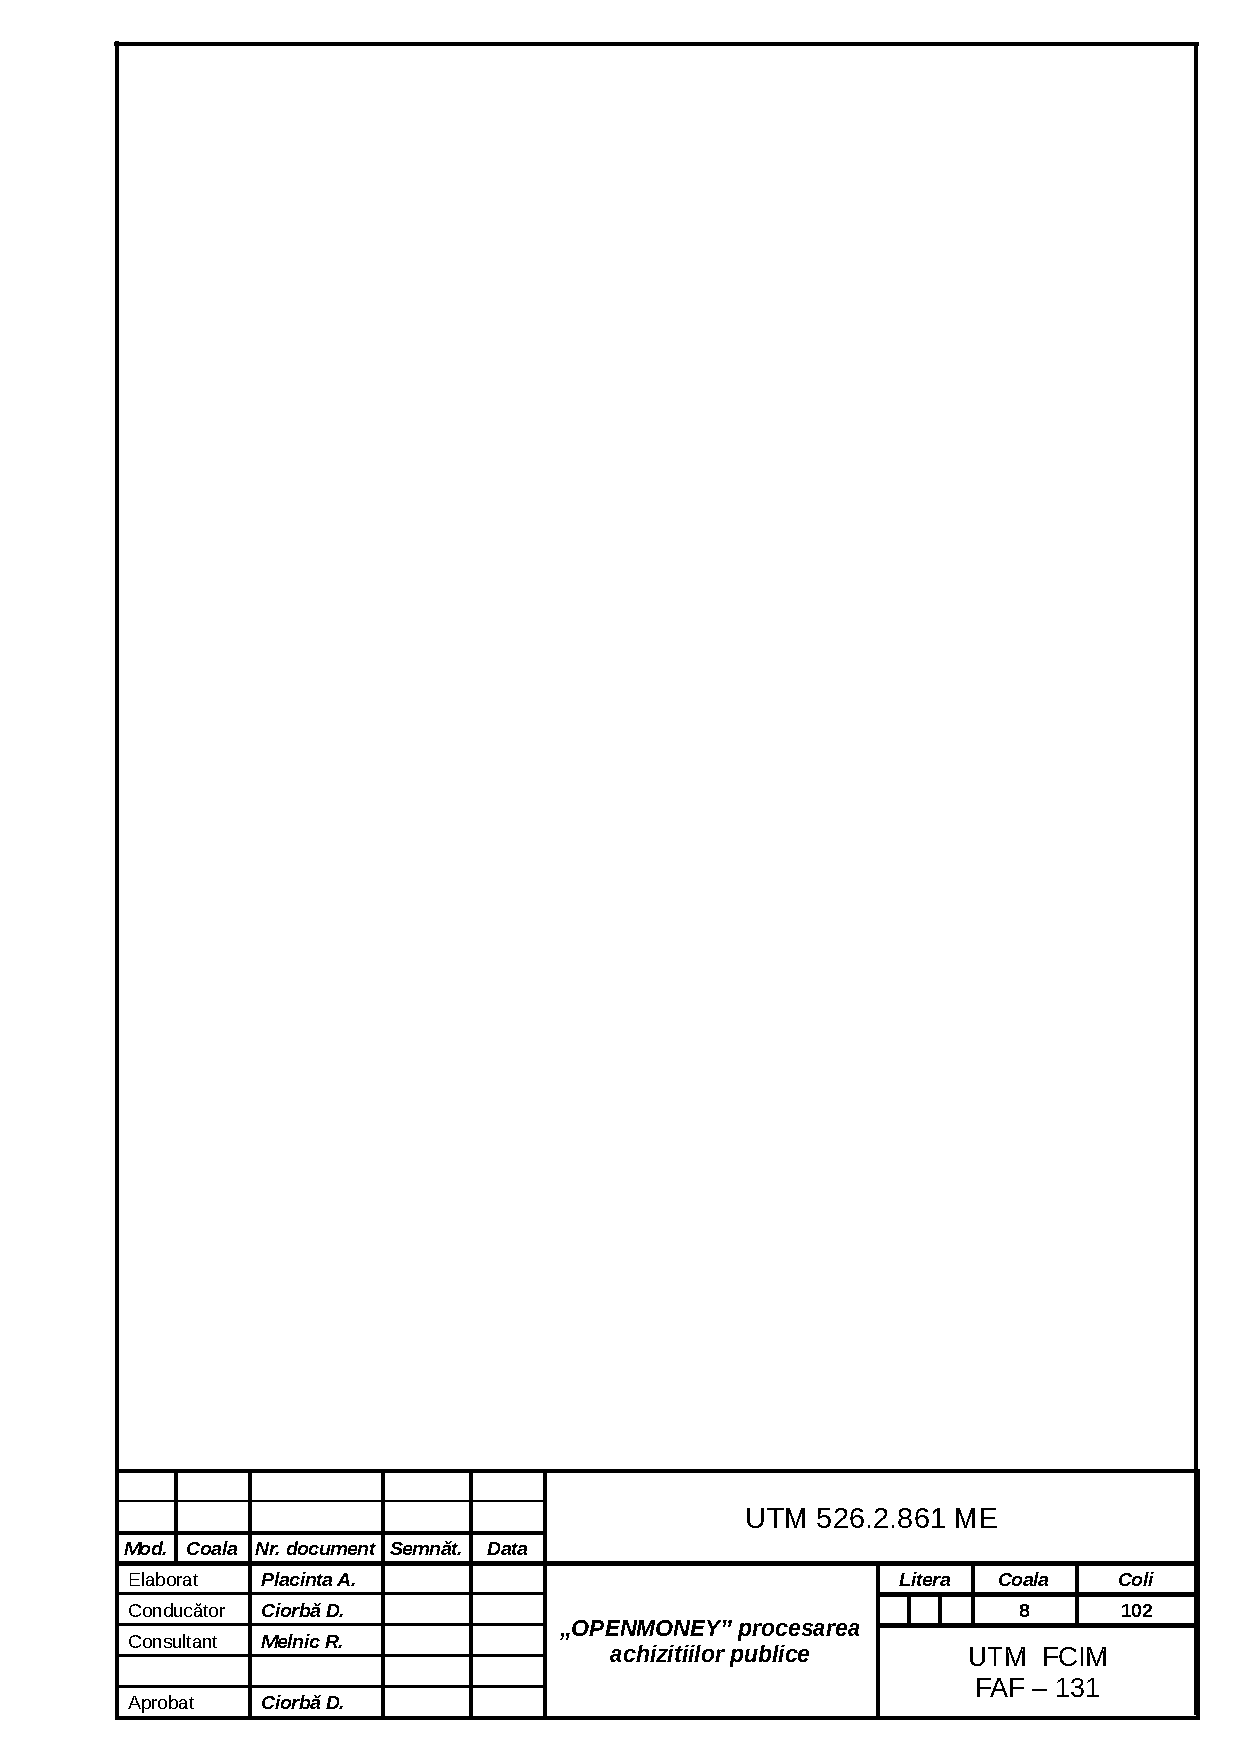
\includegraphics{Front/Chenar-Indicatori-1.pdf}}
}
\tableofcontents
\AddToShipoutPicture*{
\put(-4,0){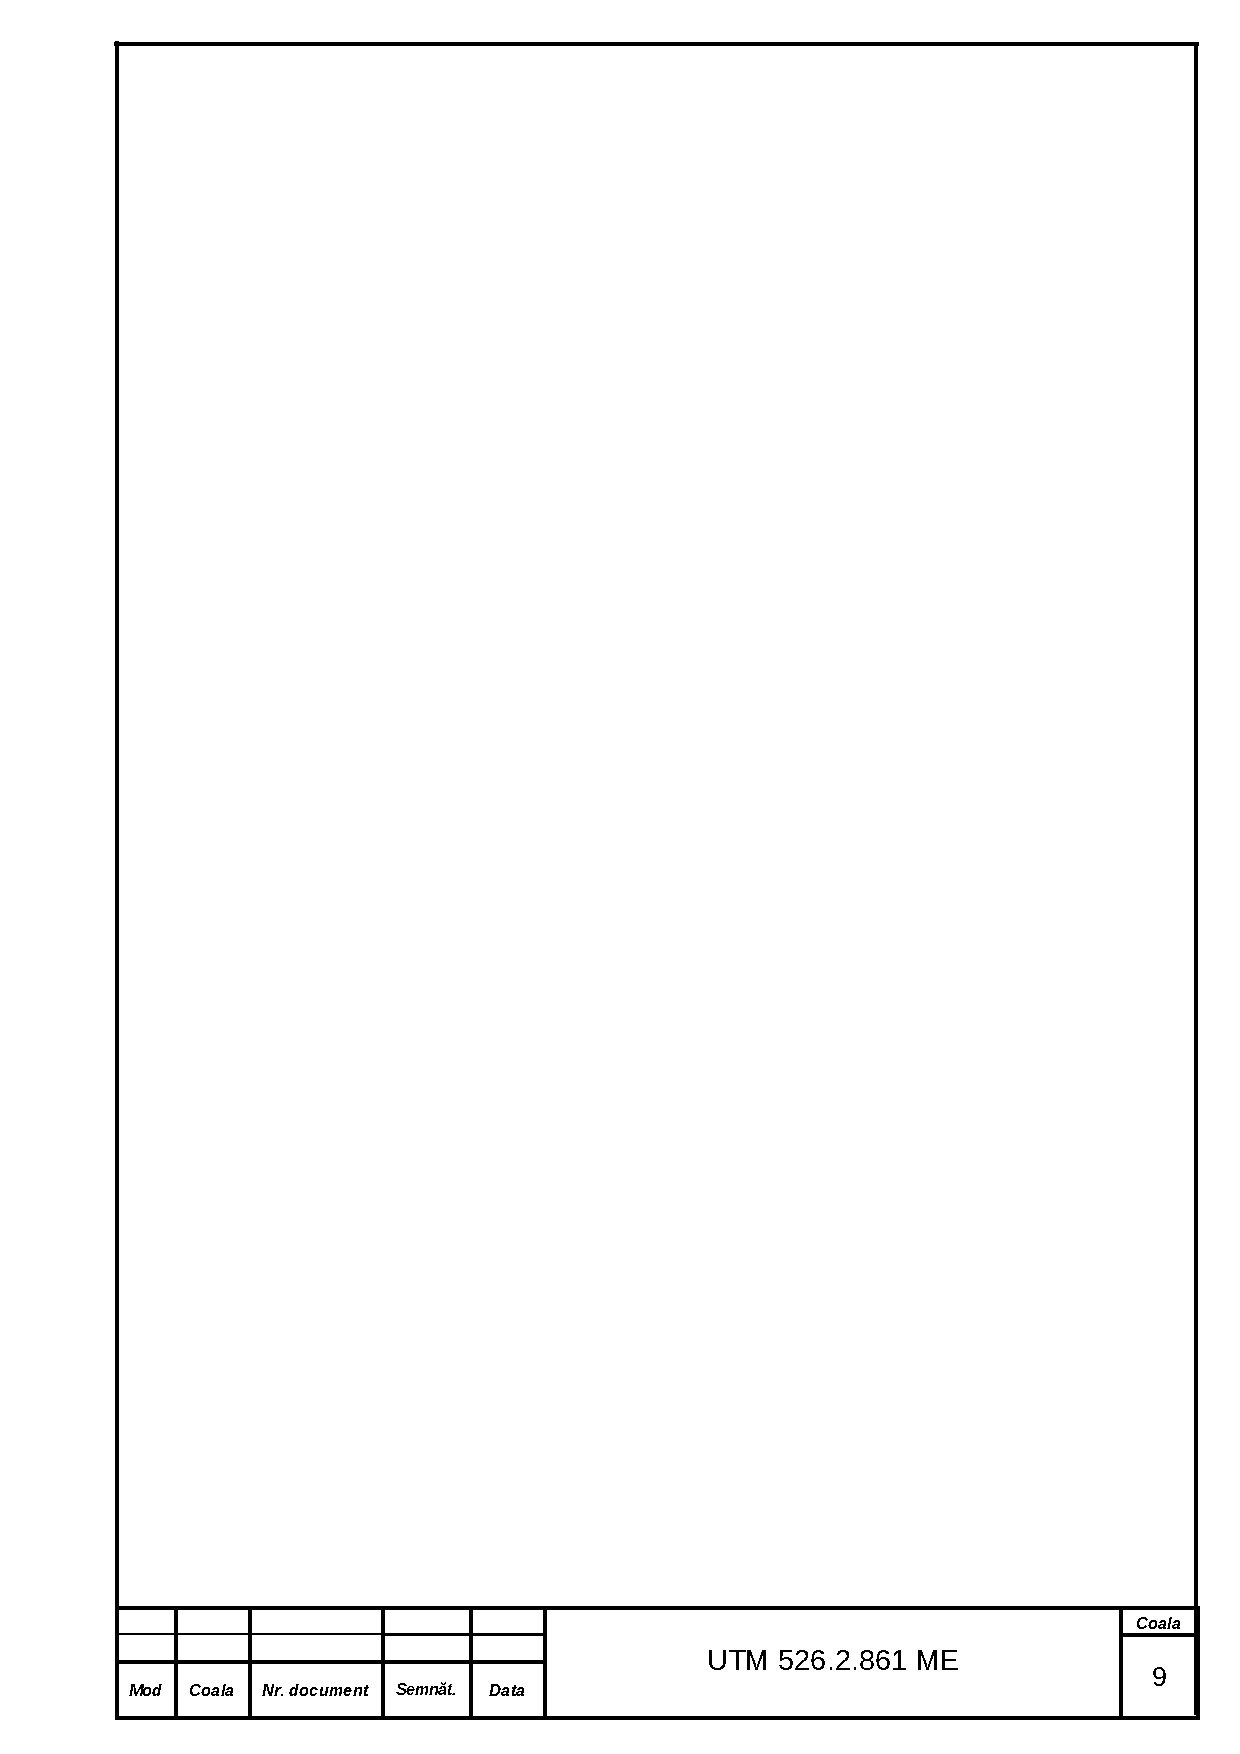
\includegraphics{Front/Chenar-Indicatori-2.pdf}}
}
\restoregeometry


\newpage
\pagenumbering{arabic}
\setcounter{page}{10}
\addcontentsline{toc}{section}{List of tables}
\listoftables
\newpage
\addcontentsline{toc}{section}{List of figures}
\listoffigures
\newpage
\addcontentsline{toc}{section}{Listings}
\lstlistoflistings
\cleardoublepage


\phantomsection
\addcontentsline{toc}{section}{Introduction}

\section*{Introduction}

	In a small group it is easy to track the actions of one or another person to keep the whole state in your mind of what is happening. In a such case you don't need extra effort to be sure in your community, but once we are trying to think in term of big society there appears a problem. People try to introduce a abstraction and try to decompose society in different groups with their own responsibility. It is hard to track the actions of such groups and in result they try to expose some reports about what they are doing. But such reports usually are hell for simple human to understand the real situation. So those all need to be processed and to show in terms more clear for human.\\

	Actually the reports are stored in a primitive structure such excel or csv. So my proposal is: first step would be to import those reports of tenders and companies into a more natural representation, and i am saying about a graph database, and the second step would be to facilitate the advantage of graph DB engine to do different kinds of processing from easiest like to visualize deep hierarchy of fondation relationships of a source company to more complicated processing like to try programatically detect posible situations of corruption: for example multiple tenders that are won by different direct companies which may be fonded indirect by the same company, or another example is how money can be stolen from a institution to a person in form of tender through a deep sequence of companies being hard to detect.\\
	
	Such application can become a tool for simple users to visualize in easy way somehow the state of what is happening and a tool for professional journalists to do a more faster analysis in this domain of tenders.\\
\cleardoublepage

\newpage
\section{Field Activity Analysis}

Data is part of everything we do, especially given the current open data movement. From financial market performance to farmer’s market locations, weather to health care, bridge and road safety to population information, significant amounts of data are yielded and available for aggregation and analysis, and can be applied to improve public services. This is the philosophy behind the open data movement —that if we make all of this data available to the public, at least the high-value data, we can crowdsource public service issues and come up with the best possible solutions. 

\subsection{IT role in data transparency}

Some definitions for Data Transparency:
\begin{itemize}
\item The ability to easily access and work with data no matter where they are located or what application created them.
\item The assurance that data being reported are accurate and are coming from the official source.
\end{itemize}

Open data is only as good as the data analytics platforms and true data transparency policies on which it relies. Bringing big data, open data and data transparency together empowers data to solve some of the world’s most challenging problems.

For researchers, public servants, data scientists and citizens to use data to spot problems and find solutions, they need big data tools to scrub and manage the data sets from their original format so they can perform investigations and operations with them. This is where the policy objectives of open data, government transparency and the technological power of big data come together. In addition, policies need to support the technology requirements. For example, while the current open data and government transparency policies allow for PDF documents to count as open data, in some cases, not all data analytics platforms can read PDF files.

The government transparency and open data movements both have the honorable goal of making data available to anyone who wants it. This isn’t just in recognition of the need to better govern, but a real step toward creating a better world. Certainly open data will improve government, but it also empowers citizens and builds economic value, not just by monetizing a resource we already have, but also by all the opportunity created from the intelligence that it enables. While the policies have paved the way, only together with big data technology will open data realize its full potential. Big data and open data are a powerful combination that can make a positive change in this world.

\subsection{Open Government Data}

Some definitions for Open Government Data:
\begin{itemize}
\item[--] Data produced or commissioned by government or government controlled entities
\item[--] Data which can be freely used, reused and redistributed by anyone.
\end{itemize}

Open data is the idea that some data should be freely available to everyone to use and republish as they wish, without restrictions from copyright, patents or other mechanisms of control. The goals of the open data movement are similar to those of other "open" movements such as open source, open hardware, open content and open access. The philosophy behind open data has been long established (for example in the Mertonian tradition of science), but the term "open data" itself is recent, gaining popularity with the rise of the Internet and World Wide Web.

Reasons for Open Government Data:
\begin{itemize}
\item[--] Transparency. In a well-functioning, democratic society citizens need to know what their government is doing. To do that, they must be able freely to access government data and information and to share that information with other citizens. Transparency isn’t just about access, it is also about sharing and reuse — often, to understand material it needs to be analyzed and visualized and this requires that the material be open so that it can be freely used and reused.
\item[--] Releasing social and commercial value. In a digital age, data is a key resource for social and commercial activities. Everything from finding your local post office to building a search engine requires access to data, much of which is created or held by government. By opening up data, government can help drive the creation of innovative business and services that deliver social and commercial value.
\item[--] Participatory Governance. Much of the time citizens are only able to engage with their own governance sporadically — maybe just at an election every 4 or 5 years. By opening up data, citizens are enabled to be much more directly informed and involved in decision-making. This is more than transparency: it’s about making a full “read/write” society, not just about knowing what is happening in the process of governance but being able to contribute to it.\\
\end{itemize}

Government data shall be considered open if it is made public in a way that complies with the principles below:
\begin{itemize}
\item[--] Complete

All public data is made available. Public data is data that is not subject to valid privacy, security or privilege limitations.
While non-electronic information resources, such as physical artifacts, are not subject to the Open Government Data principles, it is always encouraged that such resources be made available electronically to the extent feasible.

\item[--] Primary

Data is as collected at the source, with the highest possible level of granularity, not in aggregate or modified forms.

If an entity chooses to transform data by aggregation or transcoding for use on an Internet site built for end users, it still has an obligation to make the full-resolution information available in bulk for others to build their own sites with and to preserve the data for posterity.

\item[--] Timely

Data is made available as quickly as necessary to preserve the value of the data.

\item[--] Accessible

Data is available to the widest range of users for the widest range of purposes.

Data must be made available on the Internet so as to accommodate the widest practical range of users and uses. This means considering how choices in data preparation and publication affect access to the disabled and how it may impact users of a variety of software and hardware platforms. Data must be published with current industry standard protocols and formats, as well as alternative protocols and formats when industry standards impose burdens on wide reuse of the data.

Data is not accessible if it can be retrieved only through navigating web forms, or if automated tools are not permitted to access it because of a robots.txt file, other policy, or technological restrictions.

\item[--] Machine processable

Data is reasonably structured to allow automated processing.

The ability for data to be widely used requires that the data be properly encoded. Free-form text is not a substitute for tabular and normalized records. Images of text are not a substitute for the text itself. Sufficient documentation on the data format and meanings of normalized data items must be available to users of the data.

\item[--] Non-discriminatory

Data is available to anyone, with no requirement of registration.

Anonymous access to the data must be allowed for public data, including access through anonymous proxies. Data should not be hidden behind “walled gardens.”

\item[--] Non-proprietary

Data is available in a format over which no entity has exclusive control.

Proprietary formats add unnecessary restrictions over who can use the data, how it can be used and shared, and whether the data will be usable in the future. While some proprietary formats are nearly ubiquitous, it is nevertheless not acceptable to use only proprietary formats. Likewise, the relevant non-proprietary formats may not reach a wide audience. In these cases, it may be necessary to make the data available in multiple formats.

\item[--] License-free

Data is not subject to any copyright, patent, trademark or trade secret regulation. Reasonable privacy, security and privilege restrictions may be allowed.

Because government information is a mix of public records, personal information, copyrighted work, and other non-open data, it is important to be clear about what data is available and what licensing, terms of service, and legal restrictions apply. Data for which no restrictions apply should be marked clearly as being in the public domain.
\end{itemize}

\subsection{Similar systems}
After analyzing the market of data transparency projects in Moldova based on data from egov.md i highlighted two projects: \underline{bizzer.md} and \underline{idno.md}.\\

These projects together with \underline{openmoney.md} have similar functionalities to display basic information about companies with some parameters that are shown in Figure 1.1.


\begin{figure}[!ht] 
	\renewcommand\thefigure{1.1}
	\centering 
	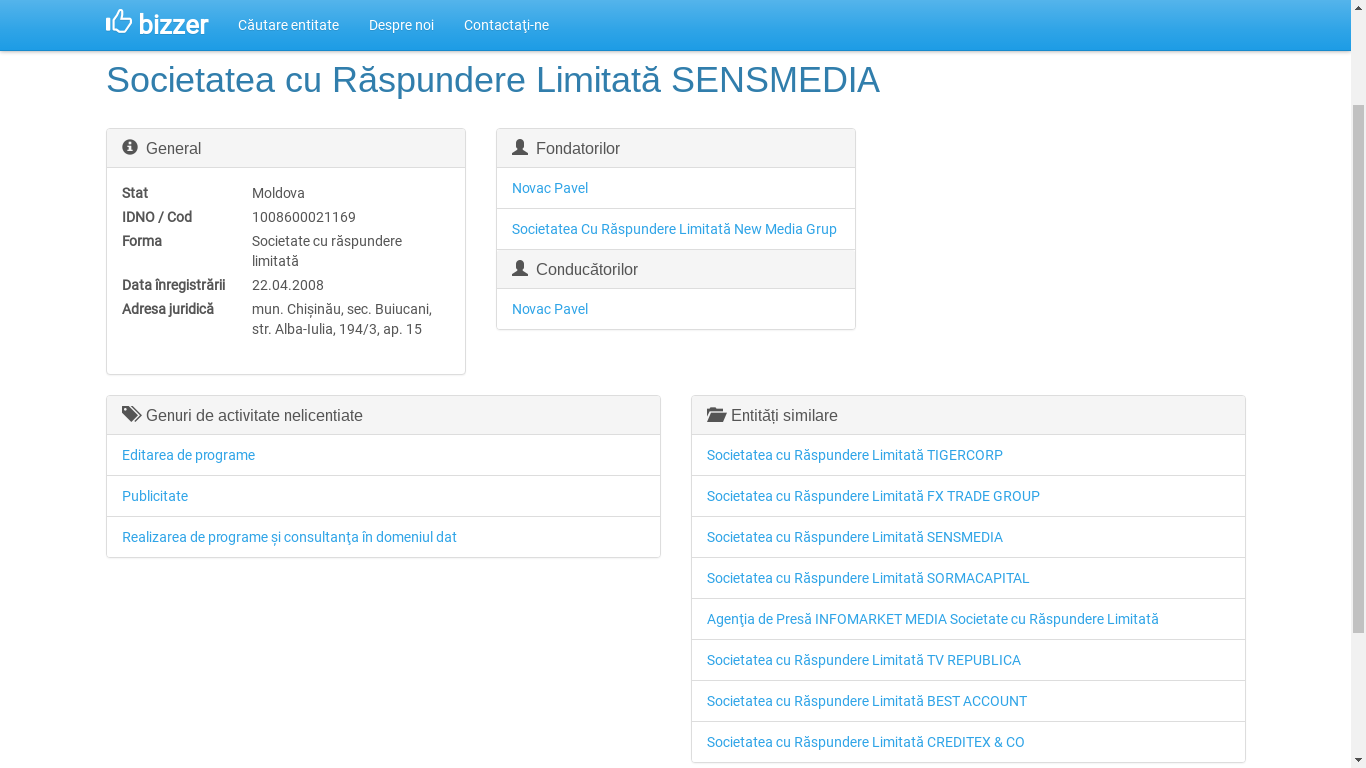
\includegraphics[width=17cm]{bizzer.png} 
	\caption{ Information about company (bizzer.md) }\label{fig}
	\end{figure}
	
\underline{idno.md} has unique feature showing all history of a company - like changing name or founders/owners that is shown in Figure 1.2.

\begin{figure}[!ht] 
	\renewcommand\thefigure{1.2} % Make this Figure I.3 
	\centering 
	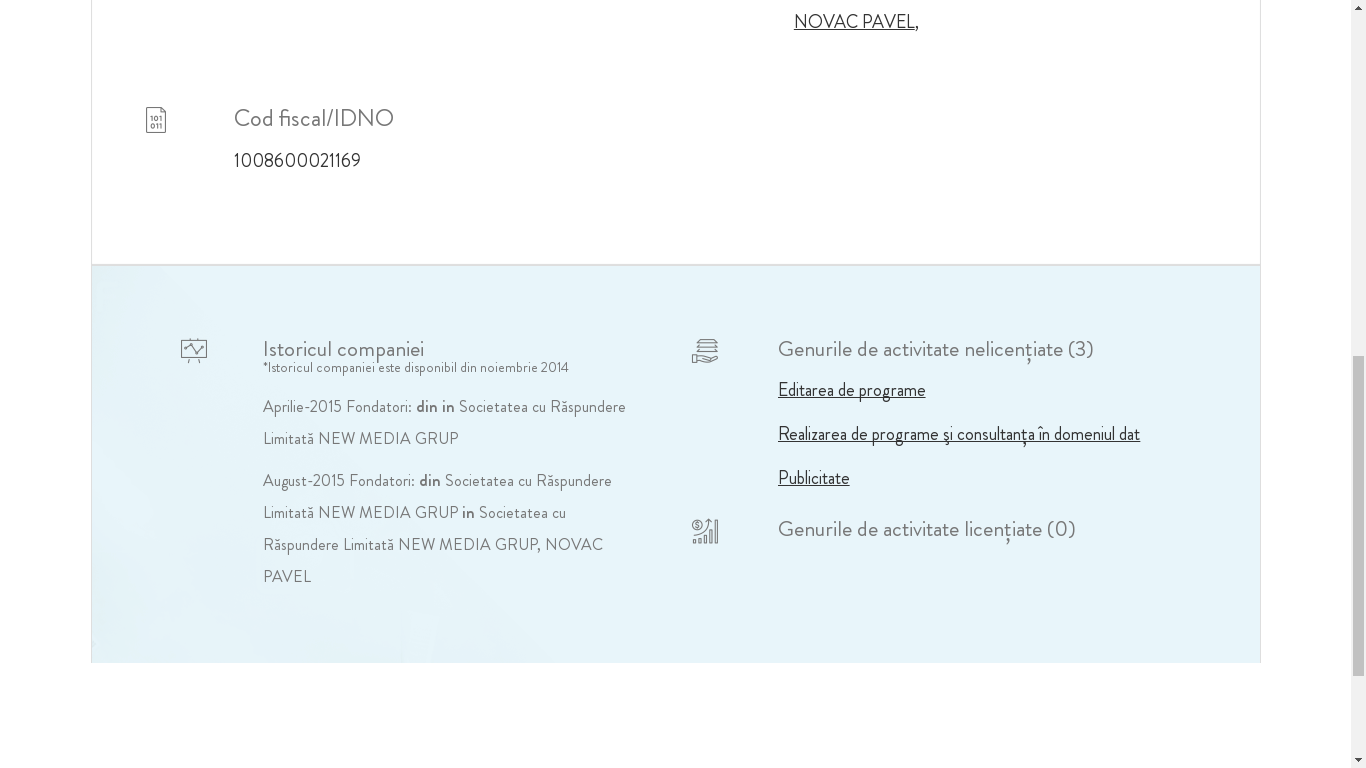
\includegraphics[width=17cm]{idno.png} 
	\caption{ History of a company (idno.md) }\label{fig}
	\end{figure}
	
	
After reviewing the structure of open government data offered by \underline{egov.md} i noticed that there are entities like companies, persons (founders and owners) and institutions. Between persons and companies exist relations (founding and ownership), also exist between institution and companies that are acquisitions. This is a perfect model for graph representation of data.\\

 So the key feature that is unique in \underline{OPENMONEY} is facilitation of graph theory in domain of open government data.\\\\\\\\\\\\\\\\\\


	\newpage
\newpage
\section{Modeling and Designing the Information System}

In this chapter will be described process of analysis, designing and development of the system.

\subsection{Analysis of project}
UML (Unified Modeling Language) is a standard notation for the modeling of real-world objects
as a first step in developing an object-oriented design methodology. Its notation is derived from and
unifies the notations of three object-oriented design and analysis methodologies:

\begin{itemize}
\item[--] Methodology for describing a set of objects and their relationships
\item[--] Object-Modeling Technique
\item[--] Approach which includes a use case methodology
\end{itemize}

Among the concepts of modeling that UML specifies how to describe are: class (of objects),
object, association, responsibility, activity, interface, use case, package, sequence, collaboration, and
state. In general UML is a graphical language which helps to visualize, specify, construct and
document all parts of a system. Before UML software design was inconsistent and hard to share.
Software engineers were having problems with explaining and understanding different notations in
software design invented by other software architecture. In this way by creating the standarts for
different elements That’s why UML has become the international language of software development,
allowing engineers to exchange their designs freely.\\

UML uses two main diagrams types to model a system: structural and behavioral. Structure
diagrams show the things in a system being modeled. In a more technical term they show different
objects in a system. In the structural diagrams enters: composite, deployment, package, profile,
class, object and component. Behavioral diagrams shows what should happen in a system. They
describe how the objects interact with each other to create a functioning system. In the behavioral
diagrams enters: communication, use case, diagram, sequence, timing and interaction. This project
is making use of class, sequence and use case diagrams to present most parts of the design\\

\subsubsection{Definition of features for simple user and admin}
Use case diagrams specify the events of a system and their flows. They are used to gather the
requirements of a system including internal and external influences. These requirements are mostly
design requirements. So when a system is analyzed to gather its functionalities use cases are prepared
and actors are identified. Now when the initial task is complete use case diagrams are modelled to
present the outside view. So in brief, the purposes of use case diagrams can be as follows:

\begin{itemize}
\item[--] Used to gather requirements of a system.
\item[--] Used to get an outside view of a system.
\item[--] Identify external and internal factors influencing the system.
\item[--] Show the interacting among the requirements are actors.
\end{itemize}

First of all need to define the interaction of people with the system, the abilities of service and to define this from point of view of ADMIN and USER.

First of all system need some data to be imported to start to work, so we start from defining ADMIN's interaction.\\

In Figure 2.1 Admin is responsible for:
\begin{itemize}
\item prepare XLS files with information of entity to a specific format for system and upload, service will process data and import into Graph DB (OrientDB)
\item removing and changing relations or entities which was wrong imported
\end{itemize}
  , 

\begin{figure}[!ht] 
	\renewcommand\thefigure{2.1} % Make this Figure I.3 
	\centering 
	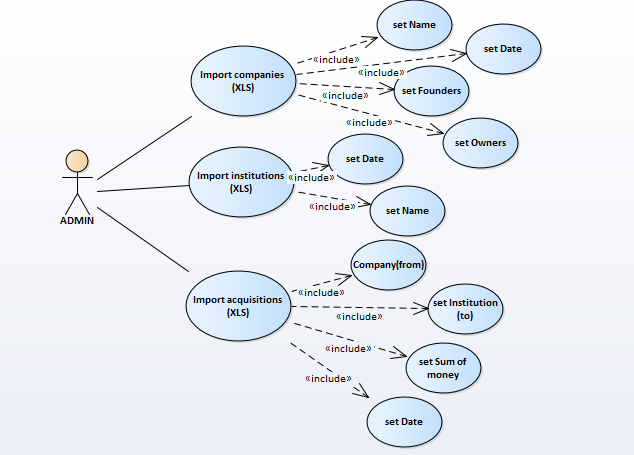
\includegraphics[width=17cm]{uc1.png} 
	\caption{ Admin's actions }\label{fig}
	\end{figure}



\newpage

In Figure 2.2 User can visualize processed data in a well exposed form:
\begin{itemize}
\item[--] Check basic info of entity, visualize hierarchy of relations in form of a graph
\item[--] View shortest paths between a person and institution (posible ways how money can distinguish from institution to a person)
\item[--] View suspicious cases where more companies have acquisitions with the same institution that have also the same founder above in hierarchy of foundation and ownership
\end{itemize}

\begin{figure}[!ht] 
	\renewcommand\thefigure{2.2} % Make this Figure I.3 
	\centering 
	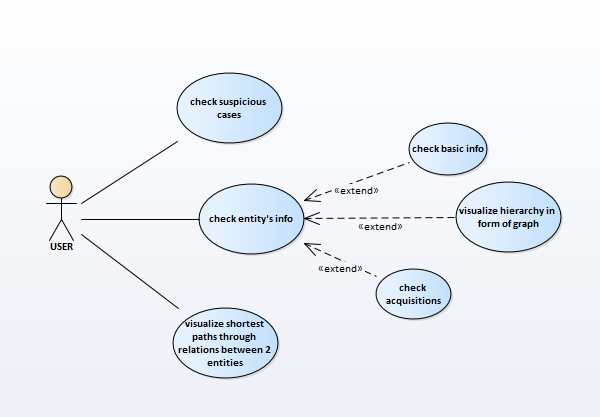
\includegraphics[width=17cm]{uc2.png} 
	\caption{ User's actions }\label{fig}
	\end{figure}



\subsubsection{Request for shortest paths between person and institution}

The Sequence Diagram models the collaboration of objects based on a time sequence. It shows
how the objects interact with others in a particular scenario of a use case. It is also a form of
interaction diagram which shows objects as lifelines running down the page, with their interactions
over time represented as messages drawn as arrows from the source lifeline to the target lifeline.
Sequence diagrams are good at showing which objects communicate with which other objects, and
what messages trigger those communications. Sequence diagrams are not intended for showing
complex procedural logic.

In Figure 2.3 is the request for shortest path and how it occure in time and how is going interaction between components like controller, service for validation of input data and data access object for retrieving the necessary data.

\begin{figure}[!ht]
	\renewcommand\thefigure{2.3} % Make this Figure I.3 
	\centering 
	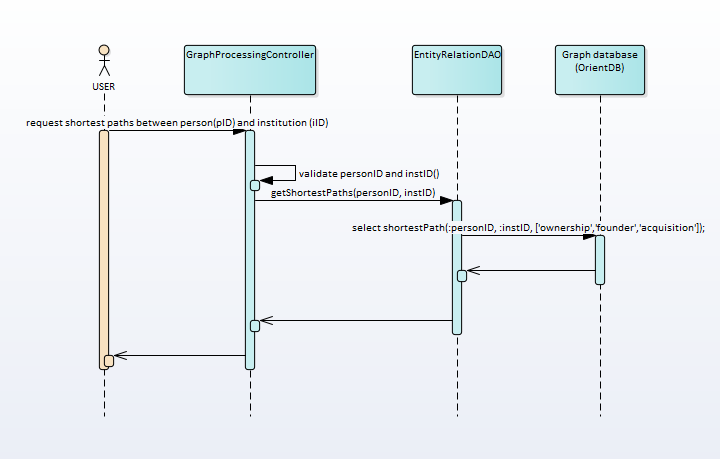
\includegraphics[width=17cm]{seq.png} 
	\caption{ User requests shortest paths between person and institution }\label{fig}
	\end{figure}


\subsubsection{Definition of class entities}
The class diagram shows the building blocks of any object-orientated system. Class diagrams
depict a static view of the model, or part of the model, describing what attributes and behavior it has
rather than detailing the methods for achieving operations. Class diagrams are most useful in illus-
trating relationships between classes and interfaces. Generalizations, aggregations, and associations
are all valuable in reflecting inheritance, composition or usage, and connections\\

Class diagram is not only used for visualizing, describing and documenting different aspects
of a system but also for constructing executable code of the software application.Class diagram is
not only used for visualizing, describing and documenting different aspects of a system but also for
constructing executable code of the software application.\\

In Figure 2.4 are represented classes used for graph processing and relationships between them, here we have one class from each layer and some classes as domain model of system.
\begin{figure}[!ht] 
	\renewcommand\thefigure{2.4} % Make this Figure I.3 
	\centering 
	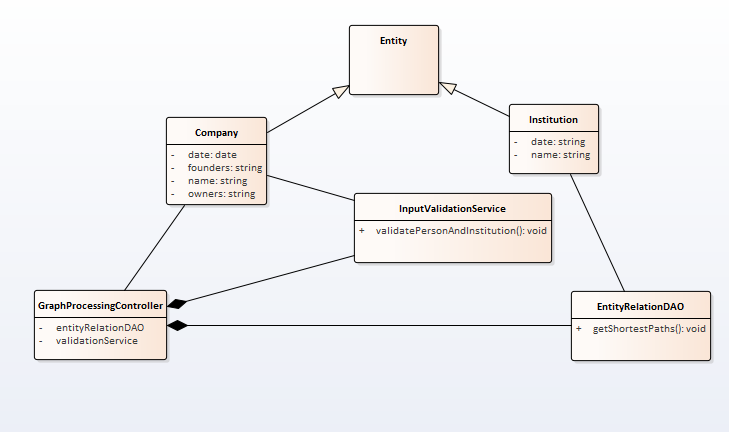
\includegraphics[width=17cm]{class.png} 
	\caption{ Class diagram }\label{fig}
	\end{figure}



\subsection{Implementation}

In this subsection will be discussed architecture of system, describing each layer with some code listings and used technologies.\\

Form-intensive enterprise class applications are ideally suited for being built as single page web apps. The main idea compared to other more traditional server-side architectures is to build the server as a set of stateless reusable REST services, and from an MVC perspective to take the controller out of the backend and move it into the browser.\\

So we can analyze system from point of view of client and server part separately, check Figure 2.5 for general architecture of system.

\newpage
\begin{figure}[!ht] 
	\renewcommand\thefigure{2.5} % Make this Figure I.3 
	\centering 
	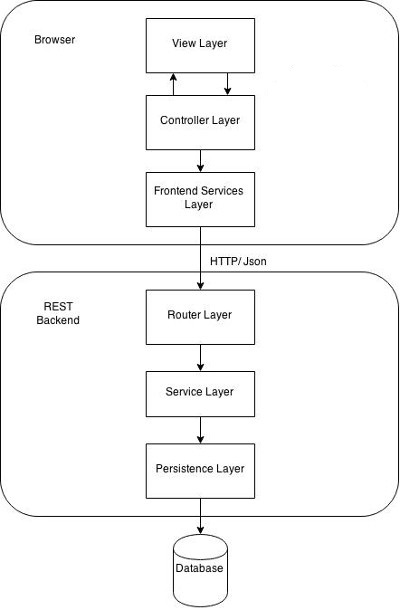
\includegraphics[width=15cm]{arch.jpg} 
	\caption{ System architecture }\label{fig}
	\end{figure}

\newpage
\subsubsection{REST backend}

The backend of an enterprise frontend application can be built in a very natural and web-like way as a REST API. The same technology can be used to provide web services to third-party applications - obviating in many cases the need for a separate SOAP web services stack.

From a DDD perspective, the domain model remains on the backend, at the service and persistence layer level. Over the wire only DTOs go by, but not the domain model.

The backend is built using the usual backend layers:
\begin{itemize}
\item Router Layer: defines which service entry points correspond to a given HTTP url, and how parameters are to be read from the HTTP request

In Listing 2.1 is controller that is used for validating of parameters from incoming request for getting shortest paths between 2 entities and delegate service components with business logic for processing that stuff.

\lstinputlisting[language=JAVA, caption={Graph processing controller}, label=list1]{src/GraphProcessingController.java}


\item Service Layer: contains any business logic such as validations, defines the scope of business transactions

In Listing 2.2 is service which is responsible for implementing all necessary business logic for exposing shortest paths between some entities with delegating some routine tasks like retrieving data to DAO layer.

\lstinputlisting[language=JAVA, caption={Graph processing Service}, label=list2]{src/GraphProcessingService.java}

\item Persistence Layer: maps the database to/from in-memory domain objects
\end{itemize}

In Listing 2.3 is DAO element which is responsible for interaction with database to retrieve some agregated data about suspicious cases  and exposing those data to service.

\lstinputlisting[language=JAVA, caption={Element Storage DAO }, label=list3]{src/ElementStorage.java}

Also there is DB layer and in Listing 2.4 is present context configuration for database transaction objects.

\lstinputlisting[language=JAVA, caption={DB context configuration }, label=list4]{src/database.xml}

\subsubsection{Client (browser)}

The client is MVC-capable and contains all the presentation logic which is separated in a view layer, a controller layer and a frontend services layer. After the initial application startup, only JSON data goes over the wire between client and server.

The frontend should be built around a view-specific model (which is not the domain model), and should only handle presentation logic, but no business logic.

These are the three layers of the frontend:
\begin{itemize}
\item View Layer - the view layer is composed of Html templates, CSS, and any Aurelia directives representing the different UI components.

In Listing 2.5 is the html template for rendering of company page.

\lstinputlisting[language=JAVA, caption={Company HTML template }, label=list5]{src/companies.html}

\item Controller and Service layers

The controller layer is made of Angular controllers that glue the data retrieved from the backend and the view together. The controller initializes the view model and defines how the view should react to model changes and vice-versa. 

A set of Aurelia services that allow to interact with the backend and that can be injected into Aurelia controllers.

In Listing 2.6 is the service to retrieve information related to company.

\lstinputlisting[language=JAVA, caption={Company service to interact with REST }, label=list6]{src/companies.js}


\end{itemize}

\subsubsection{Used technologies}

\begin{itemize}

\item[--] BACKEND:
used technologies:
\begin{itemize}
\item Java - as main language
\item Spring DI framework for wiring and in general for management of application components
\item Spring MVC framework as web layer for request handling
\item OrientDB - nosql graph database
\item Intellij IDEA - IDE for java development from Jetbrains team
\end{itemize}

\item[--] FRONTEND:
used technologies:
\begin{itemize}
\item Javascript - as main language
\item Aurelia - javascript framework for browser application
\item Webstorm - IDE for javascript development from Jetbrains team
\end{itemize}

\end{itemize}

\begin{itemize}

\item JAVA

	Java is a general-purpose computer programming language that is concurrent, class-based, object-oriented and specifically designed to have as few implementation dependencies as possible. It is intended to let application developers 'write once, run anywhere', meaning that compiled Java code can run on all platforms that support Java without the need for recompilation. Java applications are typically compiled to bytecode that can run on any Java virtual machine (JVM) regardless of computer architecture. As of 2016, Java is one of the most popular programming languages in use,articularly for client-server web applications, with a reported 9 million developers.
	 The major characteristics of Java are:

    The created programs are portable in a network. The source program is compiled into what Java calls bytecode, which can be run anywhere in a network on a server or client that has a Java virtual machine. The Java virtual machine interprets the bytecode into code that will run on the real computer hardware. This means that individual computer platform differences such as instruction lengths can be recognized and accommodated locally just as the program is being executed. Platform-specific versions of the program are no longer needed.
    The code is robust, here meaning that, unlike programs written in C++ and perhaps some other languages, the Java objects can contain no references to data external to themselves or other known objects. This ensures that an instruction can not contain the address of data storage in another application or in the operating system itself, either of which would cause the program and perhaps the operating system itself to terminate or "crash." The Java virtual machine makes a number of checks on each object to ensure integrity.
    Java is object-oriented, which means that, among other characteristics, an object can take advantage of being part of a class of objects and inherit code that is common to the class. Objects are thought of as "nouns" that a user might relate to rather than the traditional procedural "verbs." A method can be thought of as one of the object's capabilities or behaviors.
    In addition to being executed at the client rather than the server, a Java applet has other characteristics designed to make it run fast.
    Relative to C++, Java is easier to learn.
    Java was introduced by Sun Microsystems in 1995 and instantly created a new sense of the interactive possibilities of the Web. Both of the major Web browsers include a Java virtual machine. Almost all major operating system developers (IBM, Microsoft, and others) have added Java compilers as part of their product offerings.

	The Java virtual machine includes an optional just-in-time compiler that dynamically compiles bytecode into executable code as an alternative to interpreting one bytecode instruction at a time. In many cases, the dynamic JIT compilation is faster than the virtual machine interpretation.

	JavaScript should not be confused with Java. JavaScript, which originated at Netscape, is interpreted at a higher level, is easier to learn than Java, but lacks some of the portability of Java and the speed of bytecode. Because Java applets will run on almost any operating system without requiring recompilation and because Java has no operating system-unique extensions or variations, Java is generally regarded as the most strategic language in which to develop applications for the Web.


\item Spring DI

Java components / classes should be as independent as possible of other Java classes. This increases the possibility to reuse these classes and to test them independently of other classes(Unit Testing). To decouple Java components from other Java components the dependency to a certain other class should get injected into them rather that the class itself creates / finds this object. A class A has a dependency to class B if class uses class B as a variable.


If dependency injection is used then the class B is given to class A via
\begin{itemize}
\item the constructor of the class A - this is then called construction injection
\item a setter - this is then called setter injection
\end{itemize}

The general concept between dependency injection is called Inversion of Control. A class should not configure itself but should be configured from outside. A design based on independent classes / components increases the re-usability and possibility to test the software. For example, if a class A expects a Dao (Data Access object) for receiving the data from a database you can easily create another test object which mocks the database connection and inject this object into A to test A without having an actual database connection. A software design based on dependency injection is possible with standard Java. Spring just simplifies the use of dependency injection by providing a standard way of providing the configuration and by managing the reference to the created objects.

The Spring Framework is a very comprehensive framework. The fundamental functionality provided by the Spring Container is dependency injection. Spring provides a light-weight container, e.g. the Spring core container, for dependency injection (DI). This container lets you inject required objects into other objects. This results in a design in which the Java class are not hard-coupled. The injection in Spring is either done via setter injection of via construction injection. These classes which are managed by Spring must conform to the JavaBean standard. In the context of Spring classes are also referred to as beans or as Spring beans.

The Spring core container:

\begin{itemize}
\item handles the configuration, generally based on annotations or on an XML file (XMLBeanFactory)
\item manages the selected Java classes via the BeanFactory
\end{itemize}

The core container uses the so-called bean factory to create new objects. New objects are generally created as Singletons if not specified differently.

In this project Spring DI is used intensively because application has layered architecture with many components. It's very helpful to use this tool for context constructing in outside using these components. It's easy to test each element and gain ensurance in quality of application.



\item Spring MVC

	The Spring Web model-view-controller (MVC) framework is designed around a DispatcherServlet that dispatches requests to handlers, with configurable handler mappings, view resolution, locale and theme resolution as well as support for uploading files. The default handler is based on the @Controller and @RequestMapping annotations, offering a wide range of flexible handling methods. With the introduction of Spring 3.0, the @Controller mechanism also allows to create RESTful Web sites and applications, through the @PathVariable annotation and other features.
	
	"Open for extension…​" A key design principle in Spring Web MVC and in Spring in general is the "Open for extension, closed for modification" principle.

Some methods in the core classes of Spring Web MVC are marked final. As a developer you cannot override these methods to supply your own behavior. This has not been done arbitrarily, but specifically with this principle in mind.

	In Spring Web MVC is possible to use any object as a command or form-backing object; so there is no need in implementing a framework-specific interface or base class. Spring's data binding is highly flexible: for example, it treats type mismatches as validation errors that can be evaluated by the application, not as system errors. Thus the developer need not duplicate the business objects' properties as simple, untyped strings in the form objects simply to handle invalid submissions, or to convert the Strings properly. Instead, it is often preferable to bind directly to business objects.

	Spring's view resolution is extremely flexible. A Controller is typically responsible for preparing a model Map with data and selecting a view name but it can also write directly to the response stream and complete the request. View name resolution is highly configurable through file extension or Accept header content type negotiation, through bean names, a properties file, or even a custom ViewResolver implementation. The model (the M in MVC) is a Map interface, which allows for the complete abstraction of the view technology. It also gives the possibility to integrate directly with template based rendering technologies such as JSP and Velocity, or directly generate XML, JSON, and many other types of content. The model Map is simply transformed into an appropriate format, such as JSP request attributes, a Velocity template model.

	In this project Spring MVC is used as core technology in the module wich responds to the clients requests. This technology not only give the possibility to create an API in less steps but also contains additional modules for working with database. One of the strongest parts that makes Spring on of the leading technologies in WEB industry is it's documentation and it's community which is raising every day.



\item OrientDB

OrientDB is an open source NoSQL database management system written in Java. It is a multi-model database, supporting graph, document, key/value, and object models, but the relationships are managed as in graph databases with direct connections between records. It supports schema-less, schema-full and schema-mixed modes. It has a strong security profiling system based on users and roles and supports querying with Gremlin along with SQL extended for graph traversal. OrientDB uses several indexing mechanisms based on B-tree and Extendible hashing, the last one is known as "hash index", there are plans to implement LSM-tree and Fractal tree index based indexes. Each record has Surrogate key which indicates position of record inside of Array list , links between records are stored either as single value of record's position stored inside of referrer or as B-tree of record positions (so-called record IDs or RIDs) which allows fast traversal (with O(1) complexity) of one-to-many relationships and fast addition/removal of new links. OrientDB is the second most popular graph database according to the DB-Engines graph database ranking.

OrientDB’s flexible Multi-Model Database contains a pure Graph Database engine compliant with the Apache TinkerPop standard.
OrientDB is incredibly fast (storing up to 120,000 records per second*). It supports schema-less, schema-full and schema-mixed modes and includes SQL among its query languages along with a custom SQL based language which reduces the learning curve for those new to OrientDB. What’s more, our graph editor makes creating and editing vertices or edges simple.

In OrientDB all Vertices and Edges are documents. You can embed documents like any other document database, but OrientDB also supports relationships. Why connect documents rather than embedding them? To avoid duplicates. The resulting database is smaller, lighter and faster, with better use of RAM resulting in more effective caching. Upon loading a tree of documents, OrientDB will assemble the entire document structure by fetching all connections transparently. With OrientDB, traversing speed is not affected by the database size. It is always constant, whether for one record or 100 billion records. This is critical in the age of Big Data!

OrientDB and MongoDB* are both NoSQL databases that share many features, though the engines are fundamentally different. While MongoDB is a pure Document Database, OrientDB is a NoSQL solution with a hybrid Document-Graph engine that adds several compelling features to the Document Database model.

This page will outline only the most important differences.

This is a JSON document representing a simplified Order. Note the “customer” property, which is embedded inside the parent Order object.


OrientDB can embed documents like any other Document Database, but it can also connect documents like a Relational Database. The main difference is that OrientDB doesn’t use the costly JOIN, but rather uses direct, super-fast links taken from the Graph Database world.

The way this transparent fetching of connections is done is one of the strong points of OrientDB. Instead of having repeated calls to the database or costly JOIN operations, a Fetch Plan is given with the query, allowing the database to return a complete graph of interconnected documents, exactly as intended, in a single operation.

MongoDB doesn’t support ACID Transactions.  Instead, they support Atomic Operations, so any single operation against documents is atomic. This means that you cannot have Atomicity against multiple documents. For some use cases, this is acceptable, but in others this would be a big problem. OrientDB supports Atomic Operations as well as ACID Transactions, just like the Relational Database model. OrientDB uses a Write Ahead Logging (WAL) Journal to make all the changes durable, even in the event of failure.

MongoDB has its own Query Language based on JSON, which requires training to learn a new language. OrientDB’s query language is built on SQL and is augmented with a few extensions to manipulate trees and graphs.  Considering most developers are familiar with SQL, working with OrientDB is easier.

The entire storage of MongoDB is managed using the Memory Mapping technique. This is great, because it’s very fast and managed by the Operating System (OS). In the past, OrientDB used the exact same technique with its “LOCAL” Storage Engine. However, the problem with the Memory Mapping approach is that each OS manages Memory Mapped files in a different way and the available tools to tune the process are very limited and low level. This introduces many problems when databases require more space than the available RAM on the server.

In this project OrientDB is main technology because it support graph model of storage for processing all features.


\item IntelijIDEA

	IntelliJ IDEA is a Java integrated development environment for developing computer software. It is developed by JetBrains and is getting more popular with times.

	Every aspect of IntelliJ IDEA is specifically designed to maximize developer productivity.
Together, powerful static code analysis and ergonomic design make development not only productive but also an enjoyable experience.
After IntelliJ IDEA's index source code, it offers blazing fast and intelligent experience by giving relevant suggestions in every context: instant and clever code completion, on-the-fly code analysis and reliable refactoring tools. 
Smart code completion on the basic completion suggesting names of classes, methods, fields, and keywords within the visibility scope, the smart completion suggests only those types that are expected in the current context.
While IntelliJ IDEA is an IDE for Java, it also understands and provides intelligent coding assistance for a large variety of other languages such as SQL, HTML, JavaScript, etc., even when the language expression is injected into a String literal in Java code.

	The best part that makes this IDE better than other is about built-in tools and supported frameworks for different needs such as enterprise frameworks, tools for mobile development and web development.
Also there is no need in install additional softwares for version control because it automatically have addons for the most popular revision systems such as GIT, Mercurial ans SVN. 

\item Javascript

JavaScript, often abbreviated as "JS", is a high-level, dynamic, untyped, and interpreted run-time language. It has been standardized in the ECMAScript language specification. Alongside HTML and CSS, JavaScript is one of the three core technologies of World Wide Web content production; the majority of websites employ it, and all modern Web browsers support it without the need for plug-ins. JavaScript is prototype-based with first-class functions, making it a multi-paradigm language, supporting object-oriented, imperative, and functional programming styles. It has an API for working with text, arrays, dates and regular expressions, but does not include any I/O, such as networking, storage, or graphics facilities, relying for these upon the host environment in which it is embedded.

\end{itemize}

\subsection{Database Data Model}

The key technology used for this project is "OrientDB" NoSQL DBMS of graph type. The project is about relations between entities and investigation some sort of money flow from institution to other entity into a graph, so this is perfect case to use this DBMS to facilitate its engine of graph processing like shortest path for investigate possible money flow finding shortest relation between a person and institution, traverse hierarchy from an entity to visualize in deep its relations.

Schema is based on classes. OrientDB has two main classes E (Edge) and V (vertex), so you can create subclasses and generate schema of your database, but there is no constraints between subclasses, so schema of "Openmoney" is represented by a typical case that covers all relations in Figure 2.6, from the left of image is legend of subclasses.

\begin{figure}[!ht] 
	\renewcommand\thefigure{2.6} % Make this Figure I.3 
	\centering 
	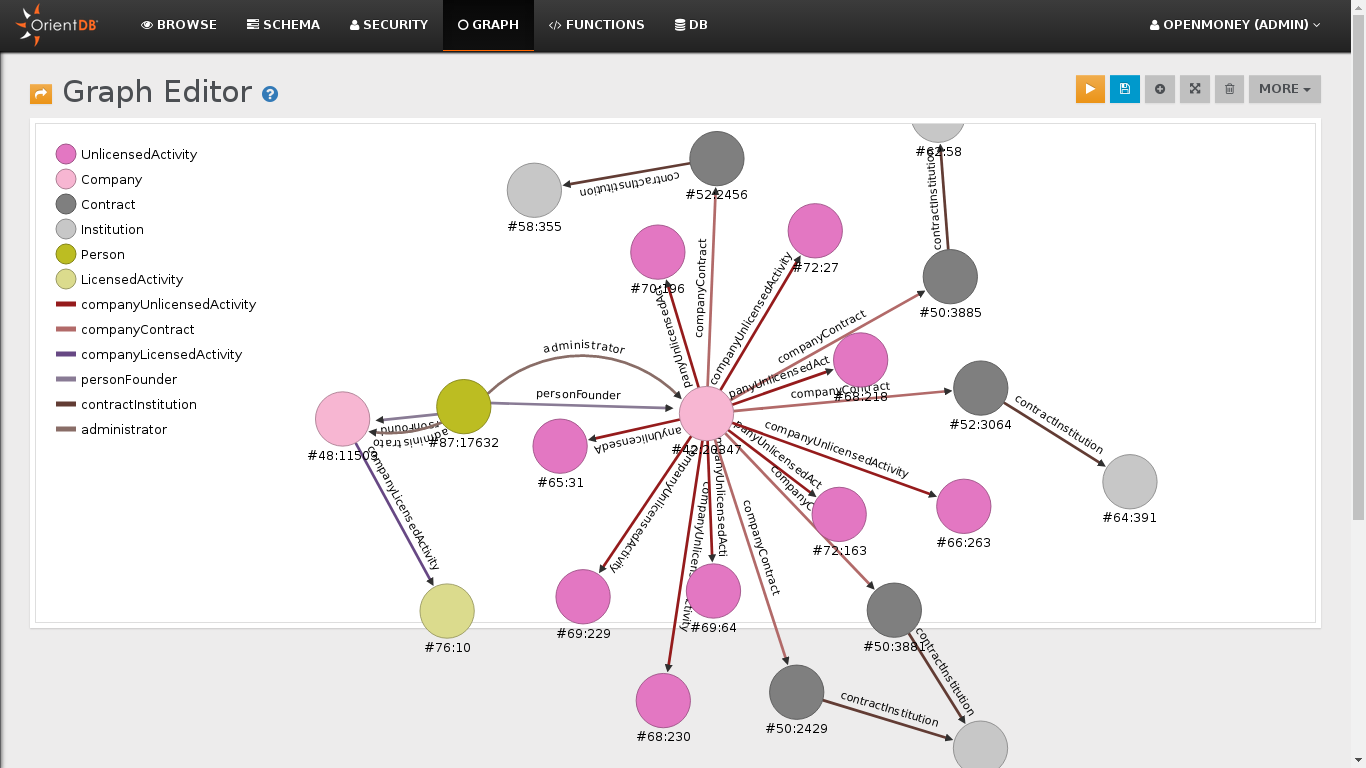
\includegraphics[width=14cm]{schema.png} 
	\caption{ Deployment diagram of server environment }\label{fig:2.5}
	\end{figure}


\subsection{Server Environment}

Deployment diagram is a structure diagram which shows architecture of the system as de-
ployment (distribution) of software artifacts to deployment targets. Artifacts represent concrete
elements in the physical world that are the result of a development process. Examples of artifacts
are executable files, libraries, archives, database schemas, configuration files, etc. Deployment target
is usually represented by a node which is either hardware device or some software execution envi-
ronment. Nodes could be connected through communication paths to create networked systems of
arbitrary complexity. In UML artifacts are deployed to nodes, and artifacts could manifest (imple-
ment) components. Components are deployed to nodes indirectly through artifacts. Deployment
diagrams could describe architecture at specification level (also called type level) or at instance level
(similar to class diagrams and object diagrams).

\begin{figure}[!ht] 
	\renewcommand\thefigure{2.7} % Make this Figure I.3 
	\centering 
	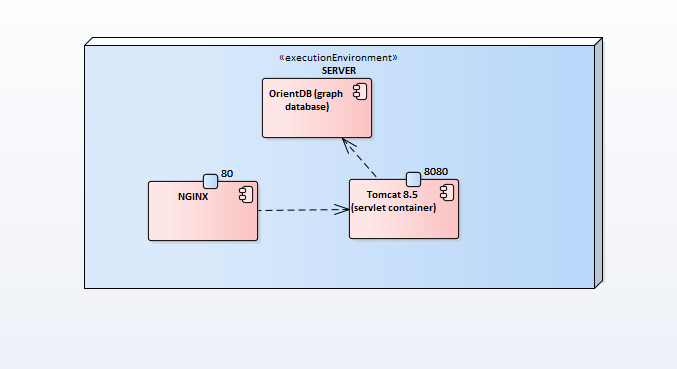
\includegraphics[width=17cm]{dep.png} 
	\caption{ Deployment diagram of server environment }\label{fig:2.5}
	\end{figure}


In server environment should be present next services (check Figure 2.7):
\begin{itemize}
\item OrientDB (NoSQL graph database)
\item Apache Tomcat - servlet container for deployment of REST service component
\item Nginx - web server as proxy to REST service for additional stuff of configuration
\end{itemize}


\newpage
\section{Review of system in action}

In this chapter, in the "Openmoney" application are analyzed already implemented features of project from client point of view.

\subsection{Home page}

In Figure 3.1 is presented Home Page with next elements:
	\begin{itemize}
	\item Total number of founders, companies and institutions existing for the last time
	\item Top 10 persons (founders or owners) by sum of contracts of direct associated companies
	\item Top 10 institutions by sum of contracts
	\item Top 10 companies by sum of contracts
	\item Random suspicious case
	\item Top 10 acquisitions by sum
	\end{itemize}

\begin{figure}[!ht] 
	\renewcommand\thefigure{3.1} % Make this Figure I.3 
	\centering 
	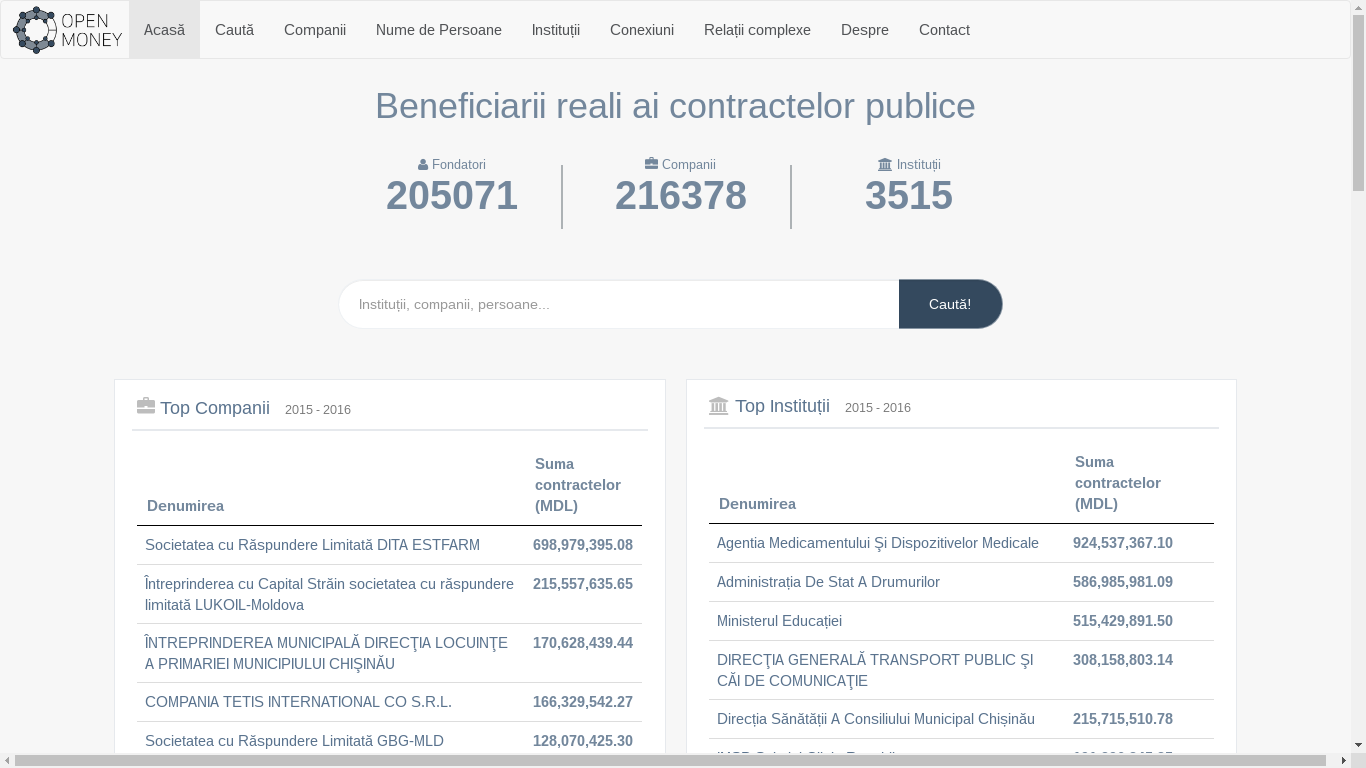
\includegraphics[width=17cm]{home.png} 
	\caption{ Home Page }\label{fig:home} 
	\end{figure}
	
\subsection{Companies}

In Figure 3.2 is default page for companies which consists a search bar where you can find a company by name or ID number of that entity and a list of top companies which stay by default. This list contains next columns: IDNO (ID of company), name, date of registration and sum of all acquisitions made by this company for period 2015-2016. Under this list you can see pagination for all companies which has at least one acquisition with state sorted by sum of money.\\

	\begin{figure}[!ht] 
	\renewcommand\thefigure{3.2} % Make this Figure I.3 
	\centering 
	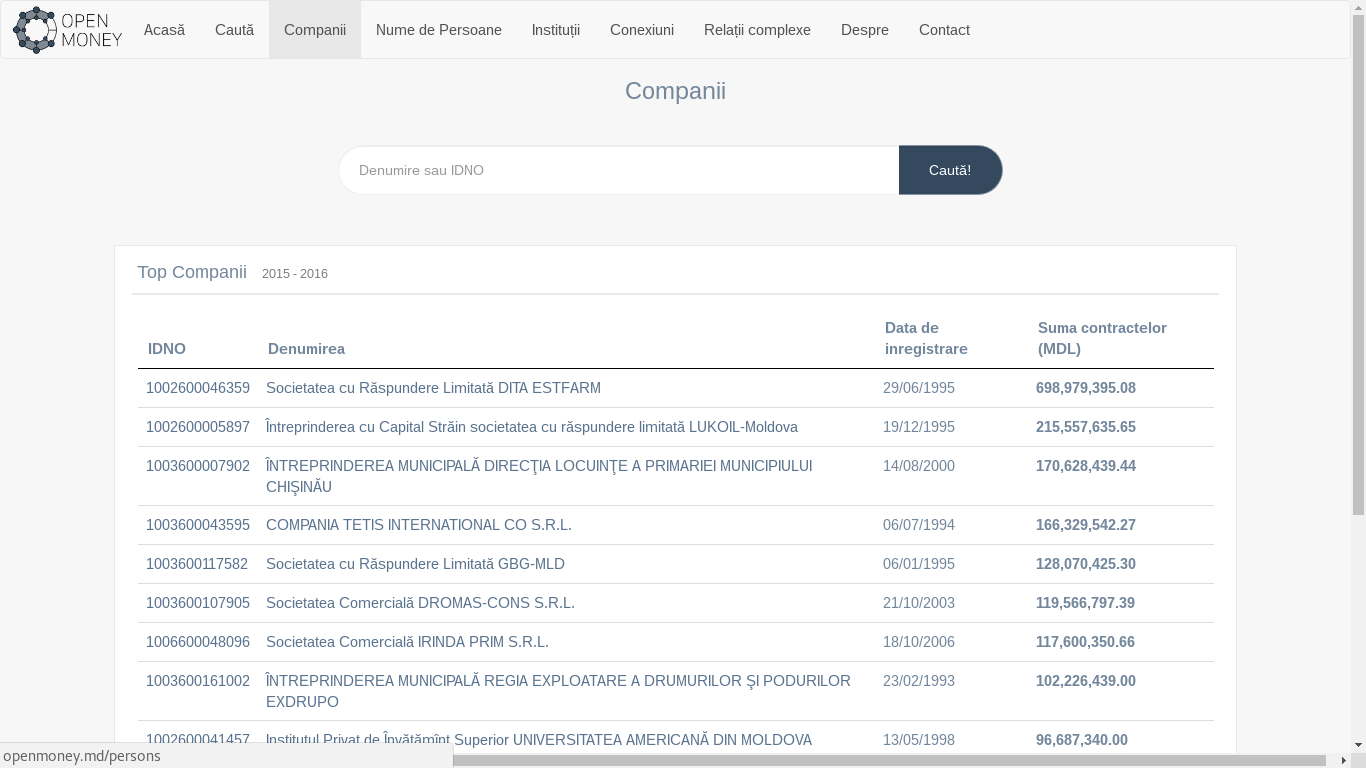
\includegraphics[width=17cm]{companies.png} 
	\caption{ Companies }\label{fig4} 
	\end{figure}
	
After clicking on necessary company user goes to another page (Figure 3.3) specific for describing that entity. This page starts from title line with name of company, after that are displaying 3 blocks with main information about company:
\begin{itemize}
\item General information - IDNO, registration date, address, state (active/inactive)
\item Organisational structure - lists with administrators and founders of that company with hyperlink to open new page with that entity
\item Activities - lists of licensed and unlicensed activities that does this company\\
\end{itemize}

	\newpage
	\begin{figure}[!ht] 
	\renewcommand\thefigure{3.3} % Make this Figure I.3 
	\centering 
	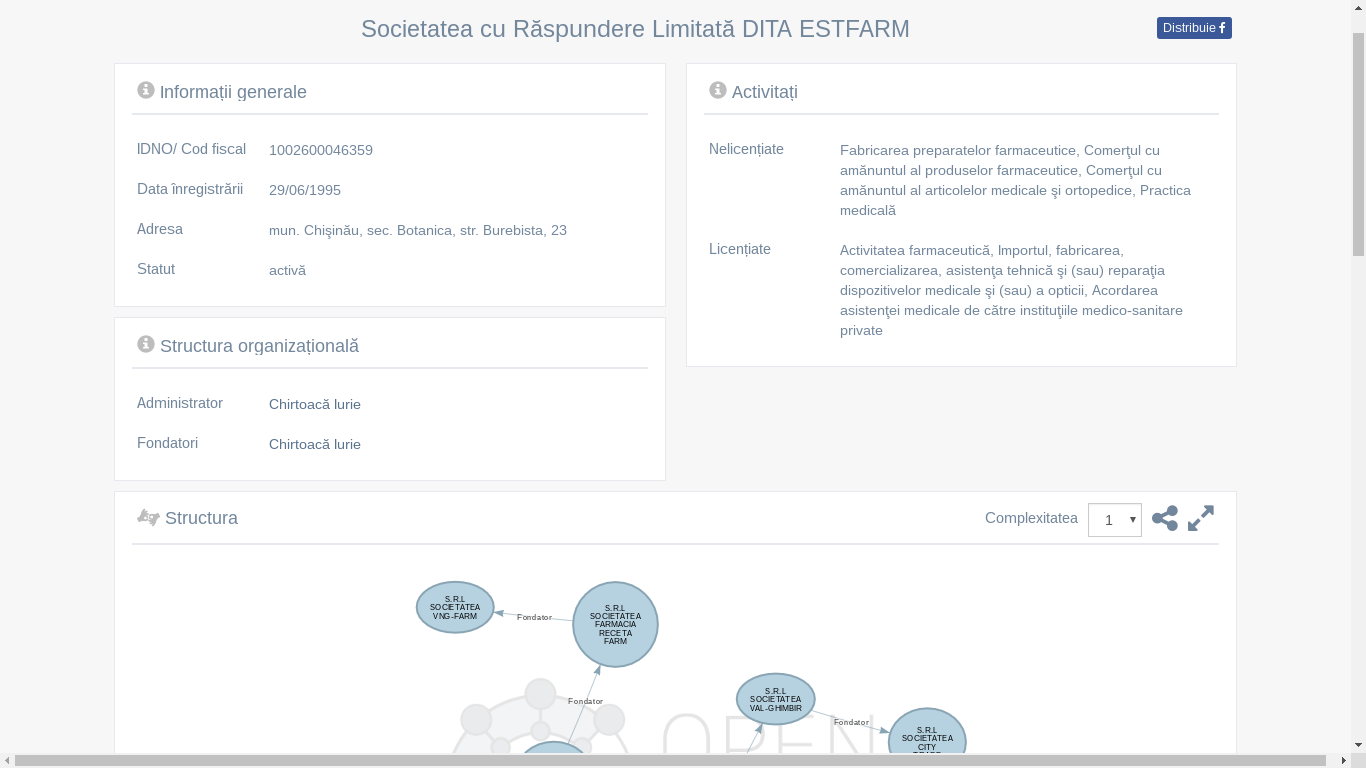
\includegraphics[width=17cm]{company_info.png} 
	\caption{ Company's main information }\label{fig4} 
	\end{figure}
	
	Next block in Figure 3.4 is visual representation of structure(hierarchy of relationship from this entity) in form of graph formed after traversing only in ONE DIRECTION (IN and OUT). There is possibility to scroll to resize canvas, to move elements, to click on entity to do check basic info and do some additional stuff. Also this block has option to change complexity(to traverse graph BIDIRECTIONAL), share as embed this graph, to swith to full screen.
	
	
	\begin{figure}[!ht] 
	\renewcommand\thefigure{3.4} % Make this Figure I.3 
	\centering 
	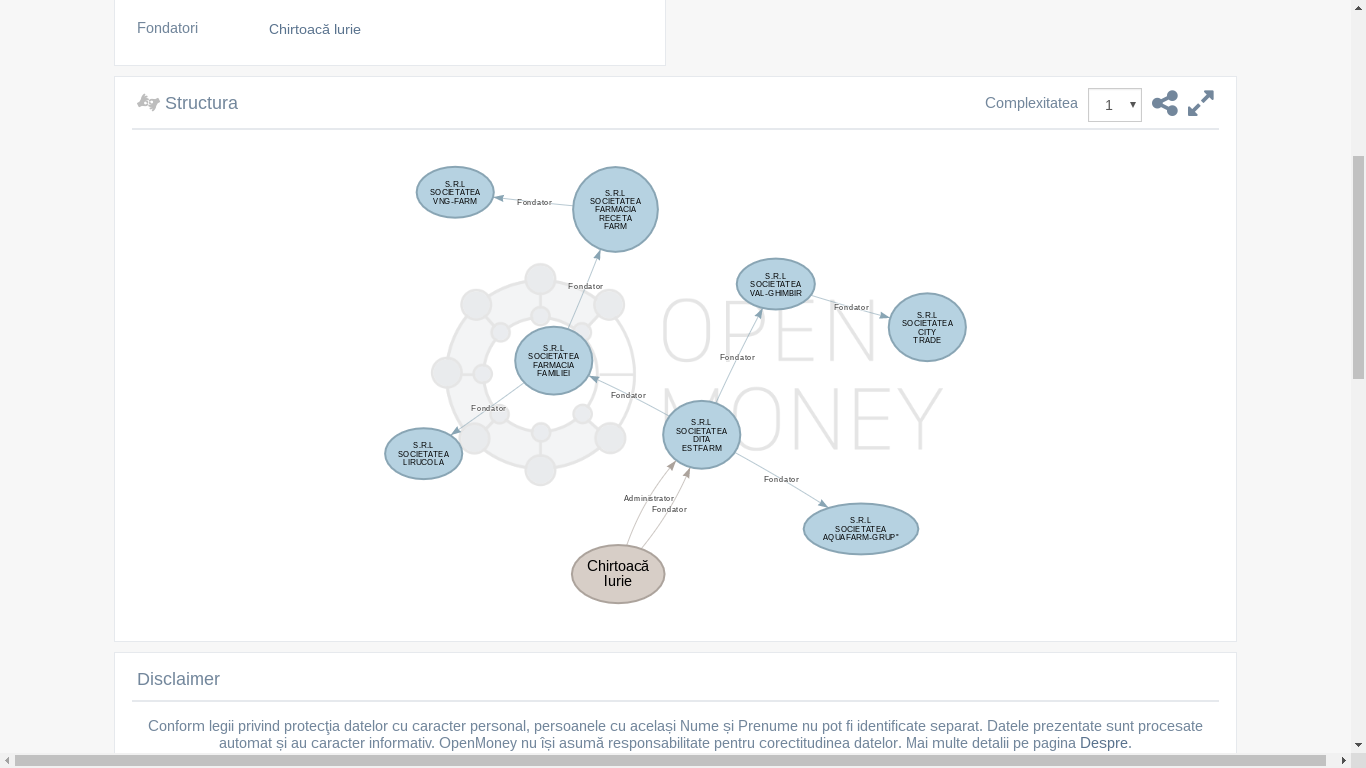
\includegraphics[width=17cm]{company_graph.png} 
	\caption{ Company's relationship structure traversing only in ONE DIRECTION}\label{fig4} 
	\end{figure}
	
	In Figure 3.5 is the last block from company page. It represents all acquisitions made by this company with pagination sorted by amount of money spent. In table are such columns as name of institutions that closed acquisitions with this company, date, type, description for exactly what was spent such amount of money and the sum.
	
	
	
	\begin{figure}[!ht] 
	\renewcommand\thefigure{3.5} % Make this Figure I.3 
	\centering 
	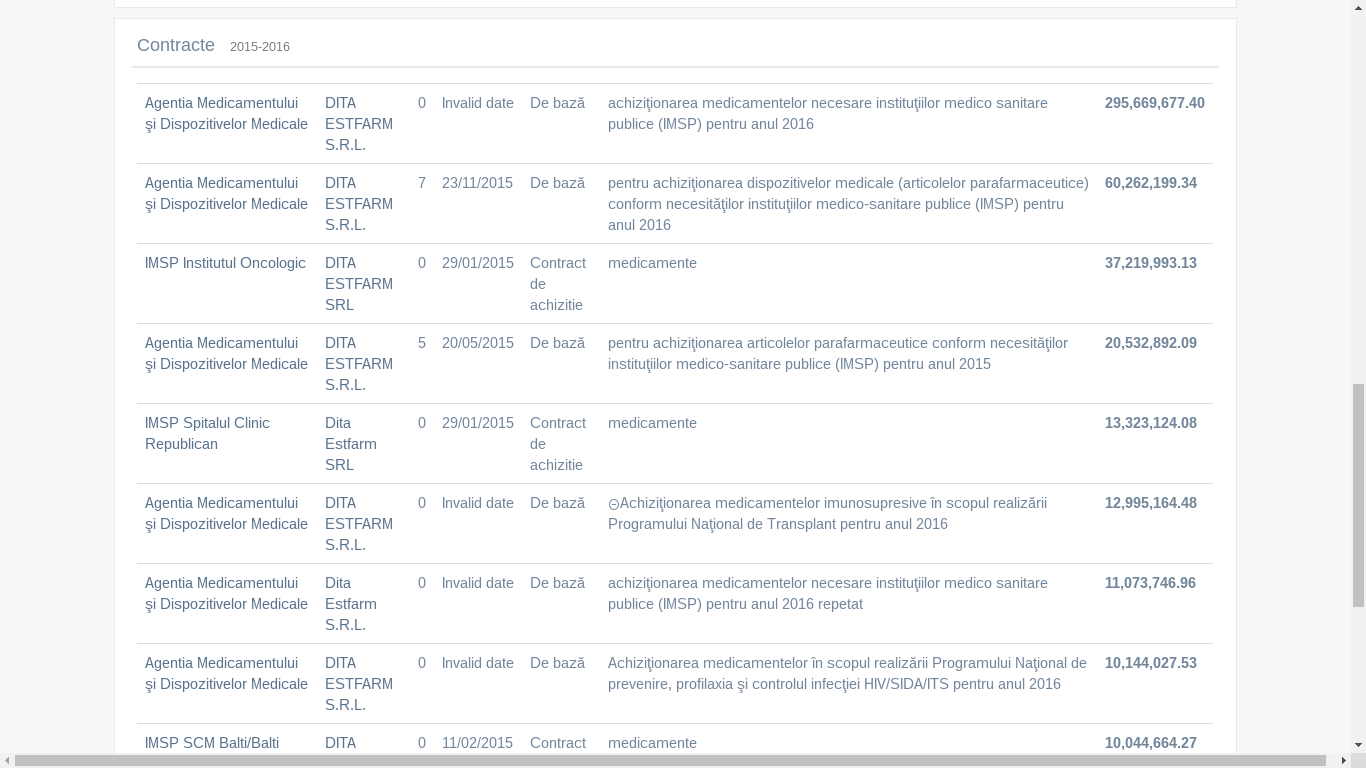
\includegraphics[width=17cm]{company_tenders.png} 
	\caption{ Company's tenders }\label{fig4}
	\end{figure}
	
	
\subsection{Persons (founders and owners)}

In Figure 3.6 is default page for persons which consists a search bar where you can find a person by name and a list of top persons which stay by default. This list contains next columns: pseudoID, name and sum of all acquisitions made by his companies for period 2015-2016. Under this list you can see pagination for all persons which has at least one acquisition with state sorted by sum of money.\\\\\\\\\\\\\\\\\\\\\\\\

	\begin{figure}[!ht] 
	\renewcommand\thefigure{3.6} % Make this Figure I.3 
	\centering 
	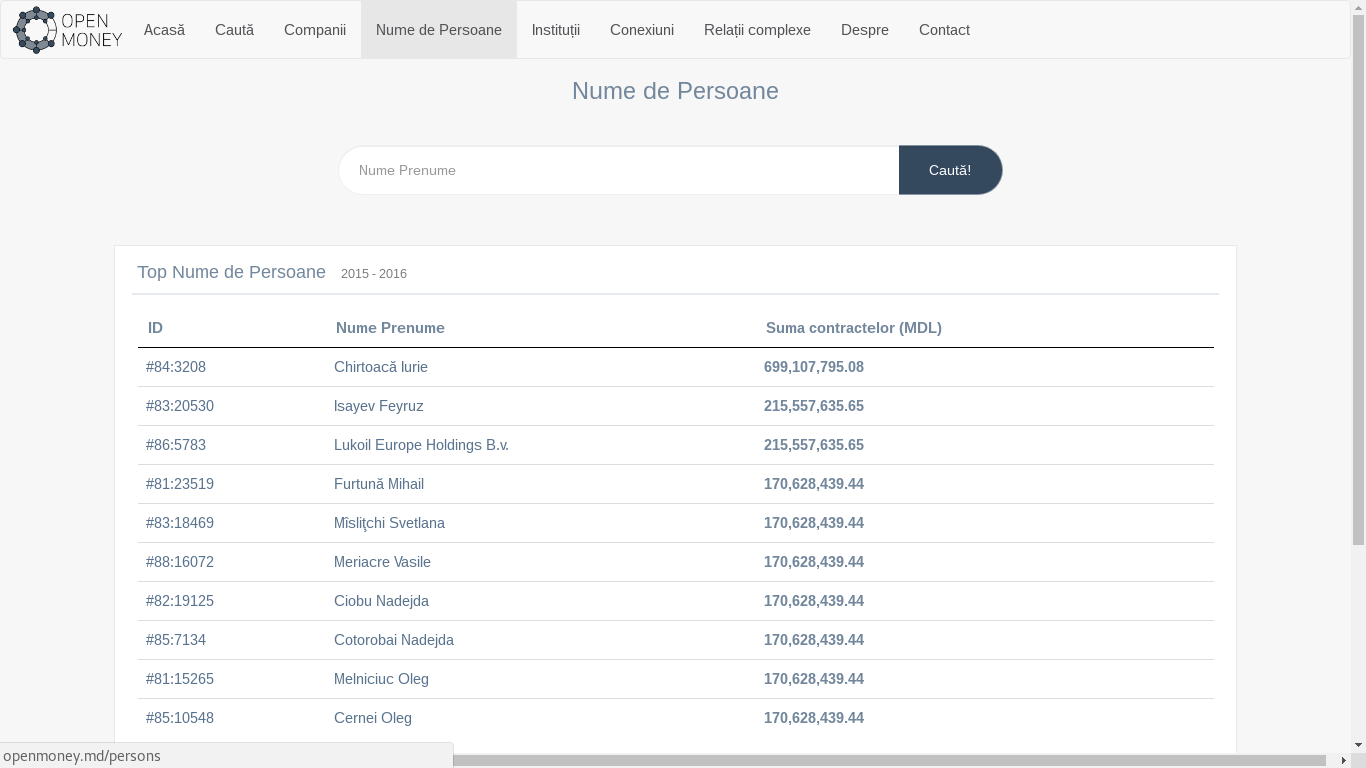
\includegraphics[width=17cm]{persons.png} 
	\caption{ Persons }\label{fig4} 
	\end{figure}
	
	In Figure 3.7 is visual representation of structure(hierarchy of relationship from this entity) in form of graph formed after traversing BIDIRECTIONAL in full screen mode.
	
	\begin{figure}[!ht] 
	\renewcommand\thefigure{3.7} % Make this Figure I.3 
	\centering 
	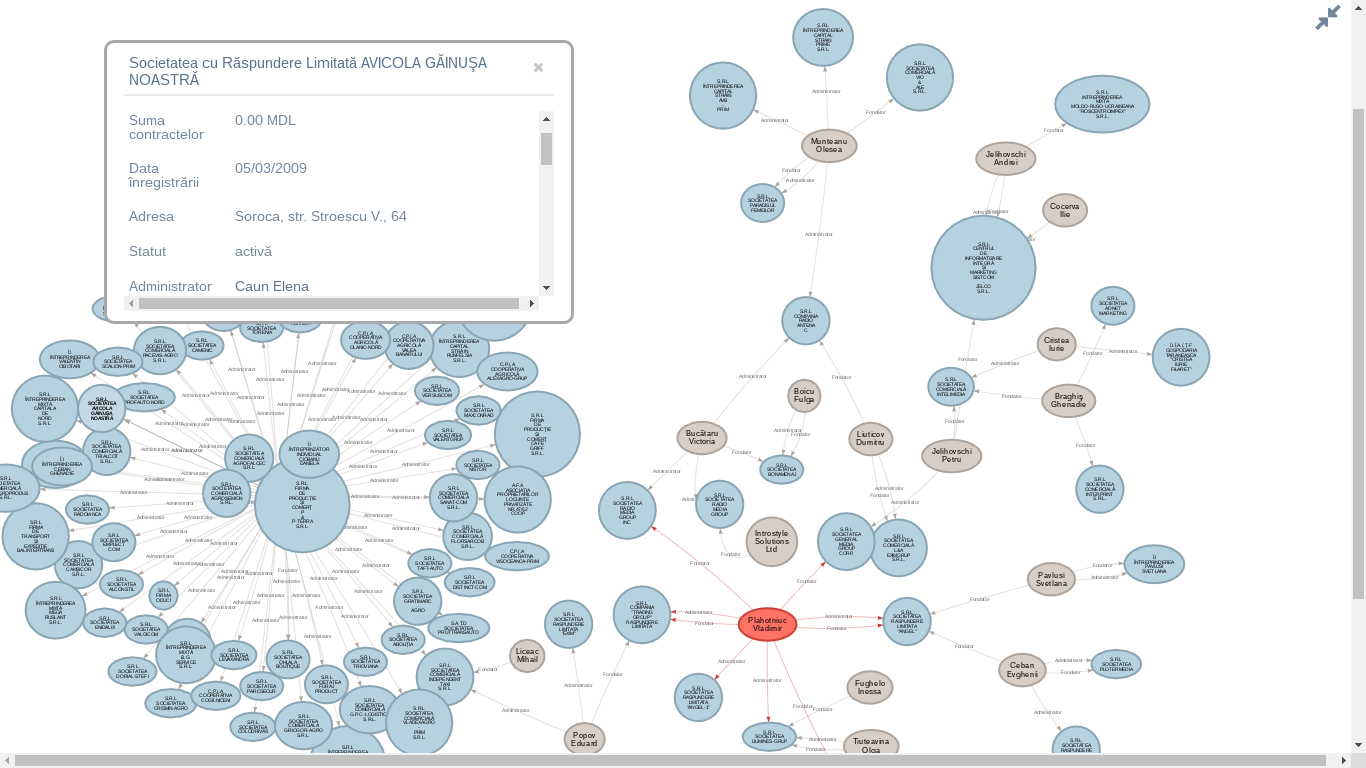
\includegraphics[width=17cm]{person_graph.png} 
	\caption{ Person's relationship structure with BIDIRECTIONAL traversing }\label{fig4} 
	\end{figure}
	
	\newpage
\subsection{Institutions}

In Figure 3.8 is default page for institutions which consists a search bar where you can find a institution by name and a list of top institutions which stay by default. 

	\begin{figure}[!ht] 
	\renewcommand\thefigure{3.8} % Make this Figure I.3 
	\centering 
	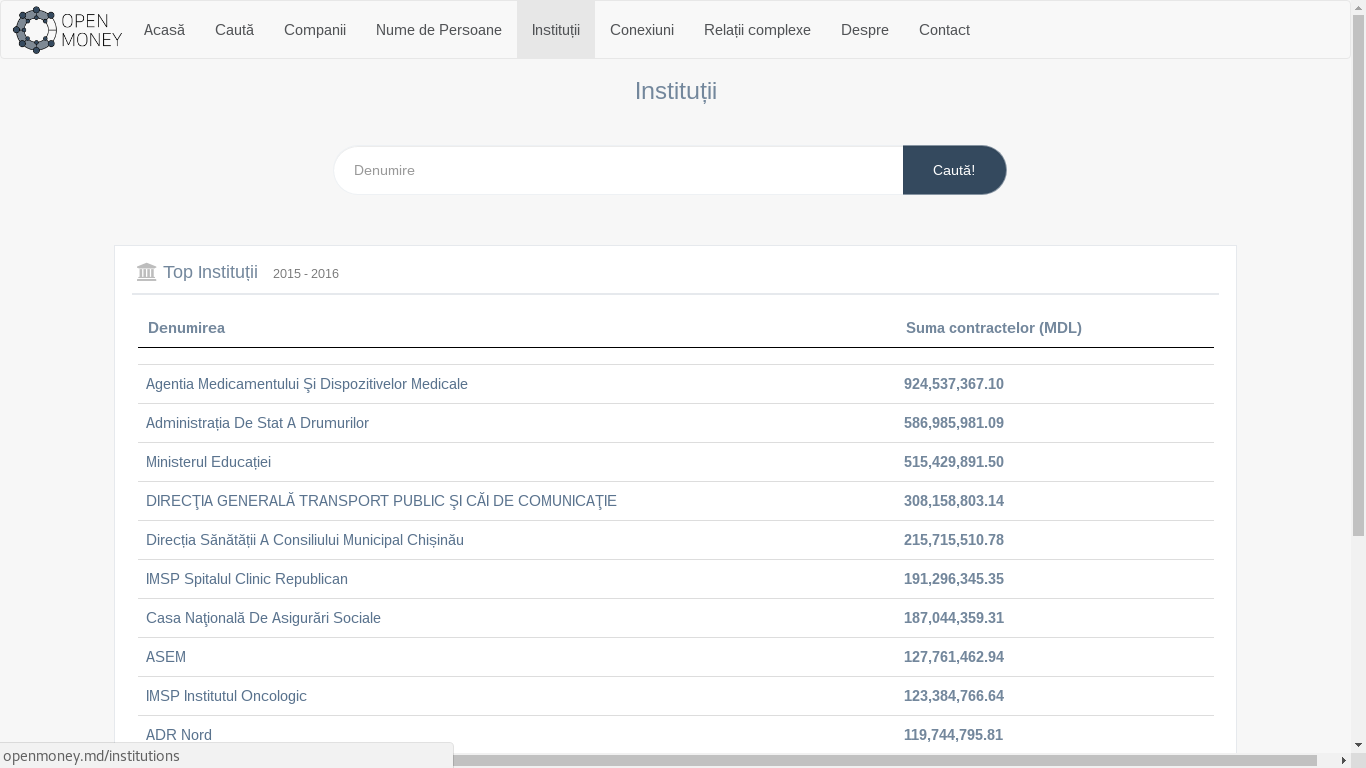
\includegraphics[width=17cm]{institutions.png} 
	\caption{ Institutions }\label{fig4} 
	\end{figure}
	
Acquisitions block in Figure 3.9. with company name and sum.

	\begin{figure}[!ht] 
	\renewcommand\thefigure{3.9} % Make this Figure I.3 
	\centering 
	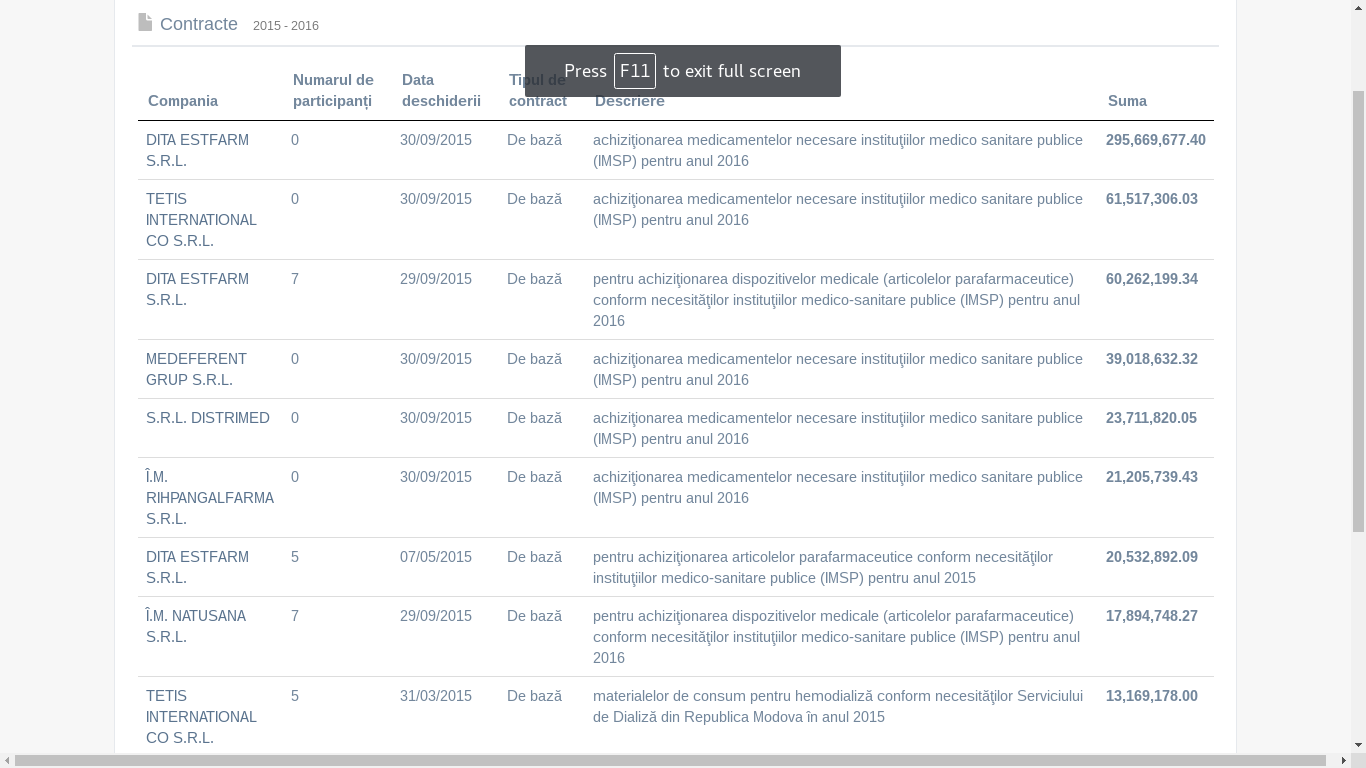
\includegraphics[width=17cm]{icontracts.png} 
	\caption{ Acquistions of an institution }\label{fig4} 
	\end{figure}
	
		\newpage
\subsection{Connections between person and institution}

In Figure 3.10 is shown "Connections" module. The idea of it is to choose a person and a institution and to try to find relations if they exist. These relations are shortest paths between companies of the person and institution through BIDIRECTIONAL relations.

Purpose of this features is to find possible money flow from an institution to a person through multiple relations that are hard to find by yourself, but is easier programmatic. Numbers under the button are size of path in sorted order.

	\begin{figure}[!ht] 
	\renewcommand\thefigure{3.10} % Make this Figure I.3 
	\centering 
	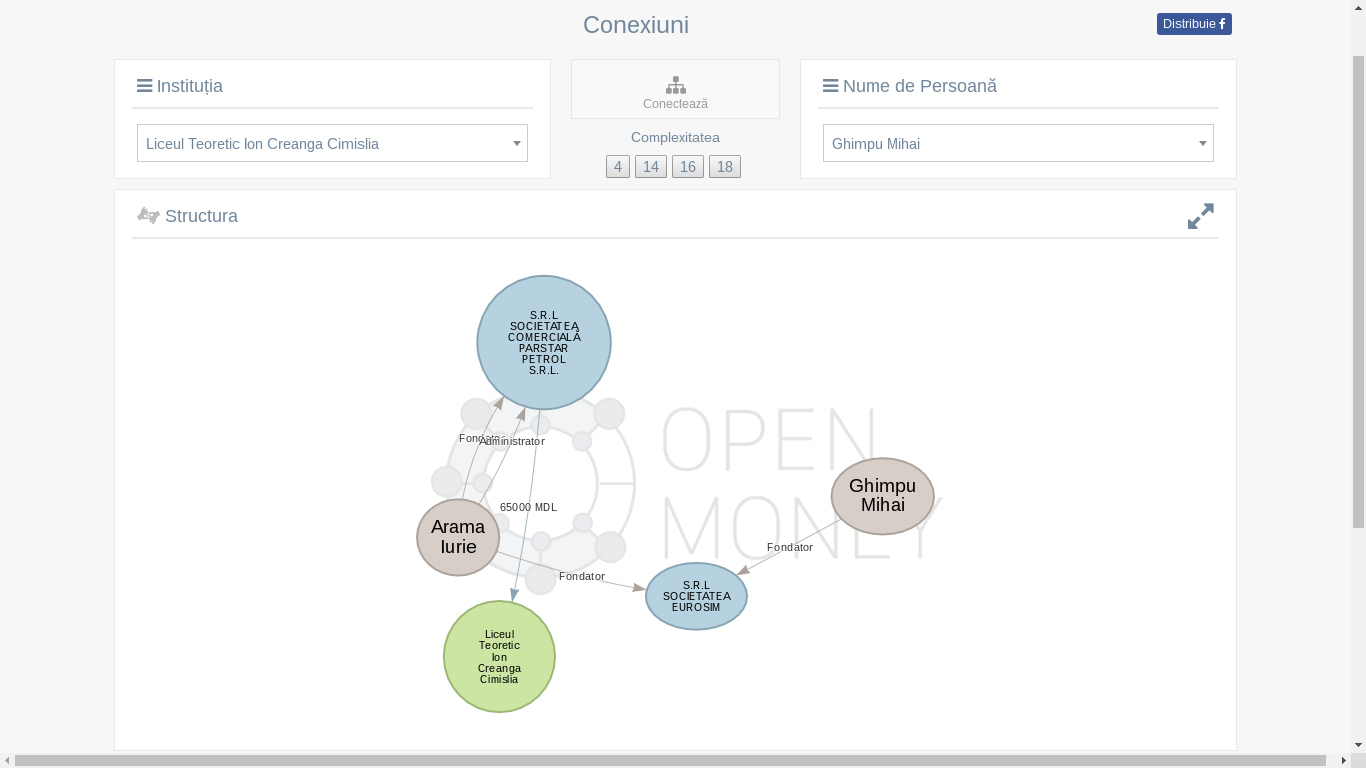
\includegraphics[width=17cm]{connections.png} 
	\caption{ Connections }\label{fig4} 
	\end{figure}
	

\subsection{Complex relation}

Complex relation - automatic detection of relation between person and institution where more companies that won tenders at the same institution are owned by same person in top level hierarchy only through DIRECTED relations, check Figure 3.11.\\

	\begin{figure}[!ht] 
	\renewcommand\thefigure{3.11} % Make this Figure I.3 
	\centering 
	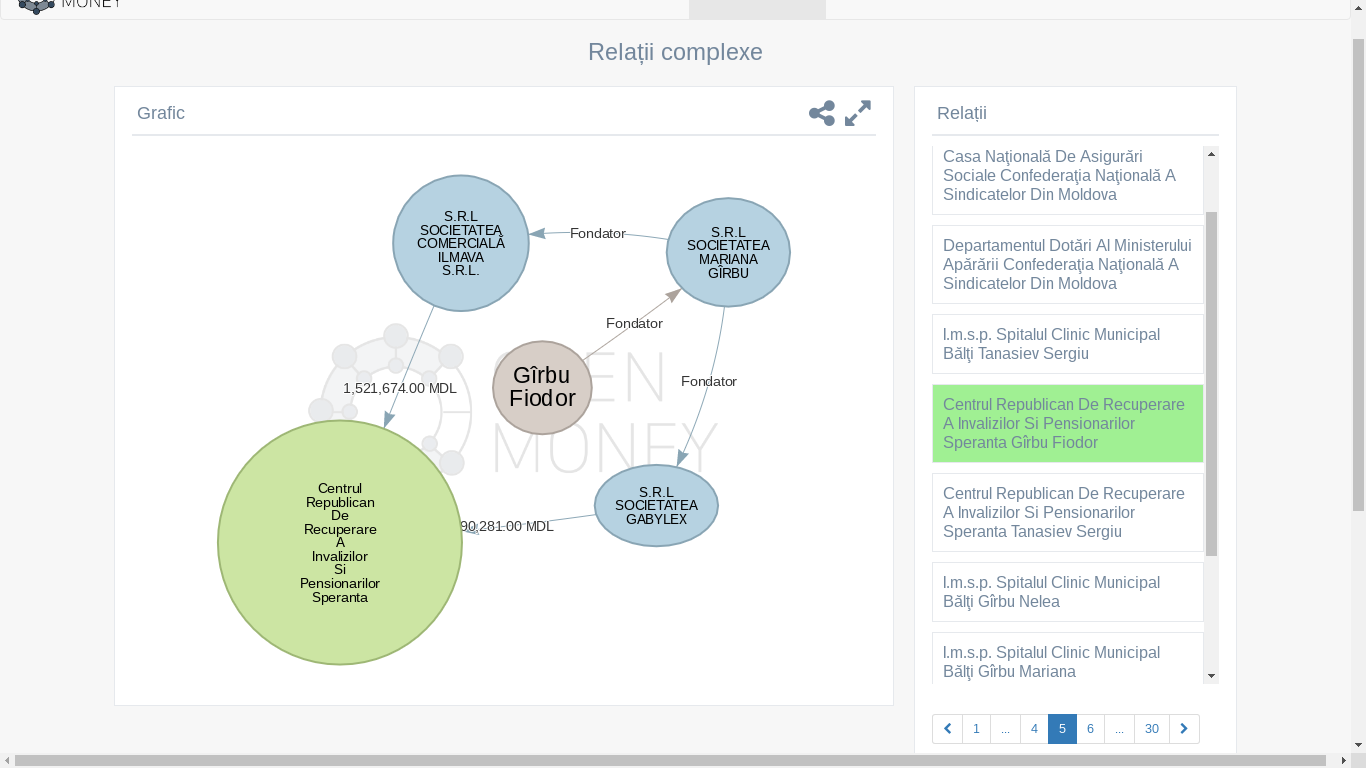
\includegraphics[width=17cm]{complex_relation.png} 
	\caption{ Complex relation  }\label{fig4} 
	\end{figure}
	
	\newpage
	\subsection{About}
	
In Figure 3.12 is a page that describes the project and show a tutorial how to use system in youtube video.	
	
	\begin{figure}[!ht] 
	\renewcommand\thefigure{3.12} % Make this Figure I.3 
	\centering 
	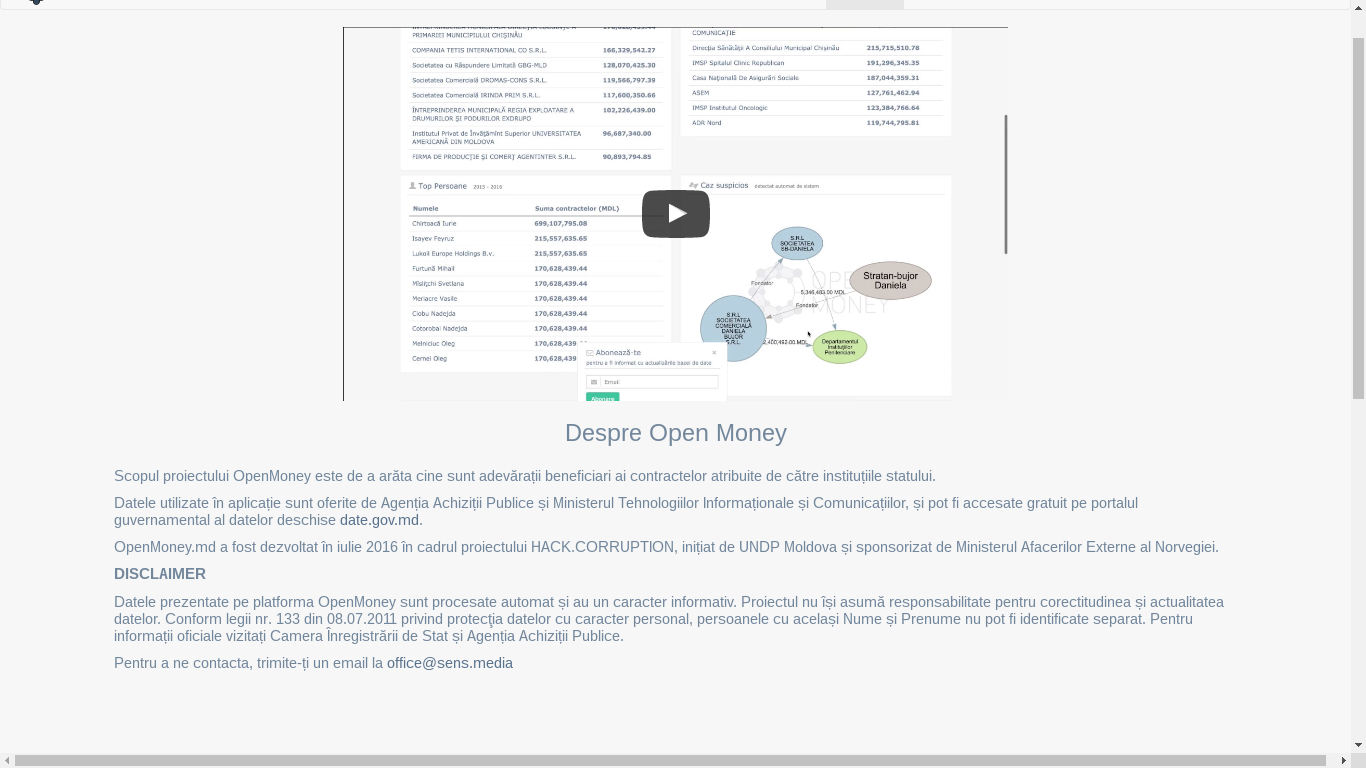
\includegraphics[width=17cm]{about.png} 
	\caption{ Page about project }\label{fig4} 
	\end{figure}
	

	



\newpage
\section{Economic Evaluation of the Project}



\subsection{Project description}

\label{section:4.project-description}

"Openmoney" is a project for visualizing information about companies and their acquisitions with institutions in a more easier way for simple users and professional journalists.

Development is based on money obtained from grant. After finishing first version need to analize the possible additional features and to try to search for other investments in dependence of wanted features.


\paragraph{Economic motivation}

The economic motivation of the project is to tend to complicated scheme analysing to find real suspicious cases, then would be possible to share this project for National anticorruption center as a service that could help them.

\subsection{SWOT Analysis}
\label{section:4.swot-analysis}
SWOT analysis or SWOT matrix is a structured planning method that evaluates Strenghs, Weaknesses, Opportunities, and Threats of a project, organization or venture. It can be applied for a wide set of topics such as a company, product, place and so on. The purpose of SWOT analysis is to investigate the internal and external factors that are favorable or unfavorable to achieve the objective. Finding respective SWOTs can be quite important, since it can reveal some later steps that are required for implementation of objective, yet only when the project has been deemed as attainable one, if not it is recommended to switch the objective that is analyzed. Yet, in order to evaluate the objective in each perspective, users of SWOT must ask and answer meaningful question that in turn generate useful information. 

\begin{table}[h]
\begin{threeparttable}
    \centering
    \caption{Analysis of project using SWOT matrix}
    \label{table:4.swot-analysis}
    \begin{tabular}{ | l | l | l | }
        \hline
        Project &   Strength    &   Weakness  \\
        \hline
            Openmoney    &
            \begin{minipage}{3in}
                \vspace{.5cm}
                \begin{itemize}
                    \item Simpler visualization of acquisitions between companies and institutions
                    \item Simpler visualization foundation and ownership hierarchy of companies
                    \item Public access for everyone
                \end{itemize}
            \vspace{.5cm}
            \end{minipage} & 
            \begin{minipage}{3in}
                \vspace{.5cm}
                \begin{itemize}
                    \item Possible errors in connections after processing
                    \item Bad structure of open data for a programmer
                    \item Special features like "connections" or "complex relation" may be misunderstood
                \end{itemize}
                \vspace{.5cm}
            \end{minipage}\\
        \hline
            Project &   Opportunities    &   Threats    \\
        \hline
            Openmoney    &
            \begin{minipage}{3in}
                \vspace{.5cm}
                \begin{itemize}
                    \item First platform of this type in Moldova
                    \item Growing interest of open data processing topics for investments
                    \item Interested institutions in additional features
                \end{itemize}
            \vspace{.5cm}
            \end{minipage} & 
            \begin{minipage}{3in}
                \vspace{.5cm}
                \begin{itemize}
                    \item Not required
                    \item No insurance in quality of data because of errors
                \end{itemize}
                \vspace{.5cm}
            \end{minipage}\\
        \hline
    \end{tabular}
    \end{threeparttable}
\end{table}

From the SWOT analysis it is clear what strenghs should application have, and currently what weaknesses should be avoided if possible. Using this analysis it is possible to foresee and plan the development accordingly, to reduce weaknesses and increase their strengths. It is important as well to monitor external changes of factors, that influence the development of product. Mostly the opportunities and threats from SWOT analysis should be used to monitor, using KPI or OCR.


There are five main steps to be accomplished in order to reach a final result for the project in discussion:
\begin{itemize}
  \item Planning (form some ideas about the design of the project, build some sketches and diagrams, determine amount of needed resources)
  \item Researching (analyze the market, the target group for which the project is intended, learn technologies for further use)
  \item Developing (create the actual system, adjust requirements to the used technologies and frameworks)
  \item Testing (perform debugging in order to ensure the well behavior of the system and integrity of functionality )
  \item Deployment (make the application available for users)
\end{itemize}

The key to a well-scheduled plan, that would lead to the in-time accomplishment of the project, is the proper subdivision of the workload, according to the given resources. Meaning that, every step enumerated above, should be scheduled for a finite period of time, judging by the level of difficulty implied. The planning period should be considered a flexible one, since at this moment some general ideas on the project have to be discussed. Changes are allowed at this step, since requirements are still established. For the researching period, it is important to be open to new ideas for consideration, in order to have a better outcome. The development period should be the most accurate one and should be divided in sprints, for better monitoring of the workflow. In the table bellow are represented all the general steps involving the development of the project. The following adnotations were used: PM – project manager, iD – developer, BD - Backend Developer.


\begin{table}[H]
\centering
\caption{Time schedule}
\resizebox{\textwidth}{!}{\begin{tabular}{| c | c | c | c |}
\hline
\textbf{Nr} & \textbf{Activity Name} & \textbf{Duration (days)} & \textbf{People involved} \\
\hline
1 & Project idea definition & 3 & PM, iD\\
\hline
2 &  Perform market analysis & 2 & PM, iD\\
\hline
3 & Establish functional features & 14 &  PM, iD \\
\hline
4 & Elaborate Use Case Diagrams & 5 & PM, iD\\
\hline
5 & Implement database design & 7 &  PM, BD\\
\hline
6 & Implement application design & 7 &  iD\\
\hline
7 & Create back-end functionality & 28 & BD\\
\hline
8 & Test back-end functionality & 4 & BD\\
\hline
9 & Develop Application & 210 & iD\\
\hline
10 & Test entire project& 7 & PM, BD, iD\\
\hline
11 & Prepare projects inside application & 3 & PM, BD, iD\\
\hline
12 & Write documentation & 7 & iD\\
\hline
13 & Upload the application to AppStore  & 2 & iD\\
\hline
14 & Commercialize the product & 3 & PM, iD\\
\hline
15 & Total time to finish the system & 302 &\\
\hline
\end{tabular}}
\label{table:schedule}
\end{table}
 
 As a generalization, Table \ref{table:schedule} represents a sketch for the first iteration of the project. Each activity was evaluated with a time stamp and responsible employees were assigned. For the completion of the purposed system including 14 activities was estimated a total amount of time including 120 working days. Bellow are indicated the amount of spent time for each individual:
 \begin{itemize}
\item PM: 44 days; 
\item BD: 49 days;
\item iD: 263 days.
 \end{itemize}

\subsection{Economic motivation}
It is actual in economy to bring economical proofs for the IT projects, basing on the specific of the concurrences in economic relationships, which suppose a wide research space. In the conditions of a low degree of determination of the marketing environment, of high prices' volatility, decreased degree of prognoses depth, a common business-plan doesn't allow the exact foreseeing of the final results of the business. In this context, one of the basic instruments is choosing the methods, the right positions and index for the economical proofs.
Realization of this goal conditions a large number of scientifically research, subordinated to the primary goal and formulated by means of the following objectives:
\begin{itemize}
\item Studying the theoretical and methodical aspects of the business-planning in the conditions of the concurrency on the market;
\item  Systematization, determining the methodology and specifying the index for the economical proof of the business-plans in IT;
\item  Study and analysis of the actual practice of economical proofs of the business-plans for IT in Republic of Moldova;
\item  Developing methodological concepts of the proofs of the decision of investment in the conditions of risk and incertitude;
\item  Studying the evaluation criteria of the business-projects' efficiency and elaboration of a mechanism of complex evaluation of these.
\end{itemize}

\subsubsection{Tangible and intangible asset expenses}
Expenses and initial budget are the ones that sharpen from the beginning the project itself, by imposing some limitations on the complexity of the system and defining its boundaries. In this section, an evaluation of the necessary amount of money will be computed, in order to ensure the correct administration of financial resources. At the beginning, in Table \ref{table:tangible_assets}, will be listed all the tangible assets used for the project. Tangible assets are defined as any assets that have a physical form. 

\begin{table}[H]
\centering
\caption{Tangible assets expenses}
\resizebox{\textwidth}{!}{\begin{tabular}{| c | c | c | c | c | c |}
\hline
\textbf{Material} &\textbf{Specification} & \textbf{Measurement unit} & \textbf{Price per unit (MDL)} & \textbf{Quantity} & \textbf{Sum (MDL)}\\
\hline
Notebook & MacBook Pro i5 2015 & Unit & 24000 & 1 &  \multicolumn{1}{r|}{24000}\\
\hline
Testing Device & iPhone 5C 16Gb & Unit & 5000 & 1 &  \multicolumn{1}{r|}{5000}\\
\hline
Cable & Original Lightning Cable & Unit & 300 & 2 &  \multicolumn{1}{r|}{600}\\
\hline
\multicolumn{5}{|r|}{Total} & \multicolumn{1}{r|}{29600}\\
\hline
\end{tabular}}
\label{table:tangible_assets}
\end{table}

The Table \ref{table:intangible_assets} presents the intangible assets, used for the project. Intangible assets are all those that do not posses a physical form. In this case, the discussion is about the \textbf{software} needed to build the application. For development was used \emph{Xcode} IDE, which requires an emph{Apple Developer Account} for deploying. For the design of UML diagrams, \emph{Enterprise Architect} was used.

\begin{table}[H]
\centering
\caption{Intangible asset expenses}
\resizebox{\textwidth}{!}{\begin{tabular}{| c | c | c | c | c | c |}
\hline
\textbf{Material} & \textbf{Specification} & \textbf{Measurement unit} & \textbf{Price per unit (MDL)} & \textbf{Quantity} & \textbf{Sum (MDL)} \\
\hline
License & Apple Developer Program & Unit & 2000 & 2 & \multicolumn{1}{r|}{4000} \\
\hline
License & Enterprise Architect Desktop Edition License & Unit & 1800 & 3 & \multicolumn{1}{r|}{5400} \\
\hline
\multicolumn{5}{|r|}{Total} & \multicolumn{1}{r|}{9400}\\
\hline
\end{tabular}}
\label{table:intangible_assets}
\end{table}

Also, additional expenses represent the direct expenses, used for work facilitation during project development. These costs cannot be included in any of the previous tables, because their values aren't included directly into the budget of the project and they have to be mentioned out of the topic. The Table \ref{table:direct_expenses} emphases the direct expenses.

\begin{table}[H]
\centering
\caption{Direct expenses}
\resizebox{\textwidth}{!}{\begin{tabular}{| c | c | c | c | c | r |}
\hline
\textbf{Material} & \textbf{Specification} & \textbf{Measurement unit} & \textbf{Price per unit (MDL)} & \textbf{Quantity} & \multicolumn{1}{c |}{\textbf{Sum (MDL)}}\\
\hline
Whiteboard & Universal Dry Erase Board & Unit & 700 & 1 & 700 \\
\hline
Paper & A4 & 100 sheets & 80 & 1 & 80 \\
\hline
Pen & Blue pen & Unit & 5 & 10 & 50 \\
\hline
\multicolumn{5}{|r|}{Total} & 830 \\
\hline
\end{tabular}}
\label{table:direct_expenses}
\end{table}

Given all the raw data, a total amount of direct expenses can be calculated: 
\begin{equation}
 T_{e} = 29600 + 9400 + 830 = 39830
\end{equation}

%\newpage
\subsubsection{Salary expenses}
In this compartment will be discussed the remuneration of each employee during the development of the project. It is assumed that each member of the team has the salary listed bellow:

\begin{itemize}
\item Project Manager – 300 MDL
\item Backend Developer – 300 MDL
\item iOS Developer – 400 MDL
\end{itemize}

After the closing of the project, some statistics regarding financial costs for employee remuneration can be presented in Table \ref{table:salaries}.

\begin{table}[H]
\centering
\caption{Salary expenses}
\resizebox{\textwidth}{!}{\begin{tabular}{| c | c | c | r |}

\hline
\textbf{Employee} & \textbf{Working days} & \textbf{Salary per day (MDL)} & \multicolumn{1}{c|}{\textbf{Salary fund (MDL)}}\\
\hline
Project Manager & 44 & 300 & 13200 \\
\hline 
Backend Developer & 49 & 300  & 14700 \\
\hline
iOS Developer & 263 & 400 & 105200 \\
\hline
\multicolumn{3}{|r|}{Total} & 133100 \\
\hline
\end{tabular}}
\label{table:salaries}
\end{table}

Besides salaries, the social service fund also retrieves a part of the money, constituting $23\%$ of total  salary. Also, there is the medical insurance fund, constituting $4,5\%$ of the same sum. The next step is to compute the social service fund, according to the relation \eqref{eq:sf} :

\begin{equation}
\label{eq:sf}
\begin{split}
 FS &= F_{re} \cdot T_{fs} \\
    &= 133100 \cdot 0.23  \\
    &= 30613,
\end{split}
\end{equation}
\noindent
where $FS$ is the salary expense, $F_{re}$ is the salary expense fund and $T_{fs}$ is the social service tax approved each year. The medical insurance fund is computed as:

\begin{equation}
\begin{split}
 MI &= F_{re} \cdot T_{mi}\\ 
    &= 133100 \cdot 0.045 \\ 
    &= 5989.5,
 \end{split}
\end{equation}

\noindent
where $T_{mi}$ is the mandatory medical insurance tax approved each year by law of medical insurance.

Now, the total work expense fund is calculated as sum of the previous computed indicators:

\begin{equation}
\begin{split}
 WEF &= F_{re} + FS + MI\\
     &= 133100 + 30613 + 5989.5 \\
     &= 169702.5,
\end{split}
\end{equation}

\noindent
where $WEF$ is the work expense fund, FS is the social fund and MI is the medical insurance fund. The final indicator shows the total work expense fund.

\subsection{Individual person salary}
Having the total work expense fund computed, it is necessary to determine the net salary for the developer. Considering the developer's salary of 400 MDL per day and there is a totally 120 working days for accomplishing the project, so the gross salary that the developer gets is:

\begin{equation}
 GS = 400 \cdot 263 = 105200,
\end{equation}

\noindent where $GS$ is the gross salary computed in MDL.

Social fund tax this year represents $6\%$, so the amount that should be tax paid in MDL represents

\begin{equation}
 SF = 105200 \cdot 0.06 = 6312.
\end{equation}

Medical insurance tax represents $4.5\%$ and gives the following result

\begin{equation}
 MIF = 105200 \cdot 0.045 = 4734.
\end{equation}

In order to proceed with income tax computations, it is necessary to calculate the amount of taxed salary.

\begin{equation}
\begin{split}
 TS &= GS - SF - MIF - PE \\
              &= 105200 - 6312 - 4734 - 10128 \\ 
              &= 84026,
\end{split}
\end{equation}

\noindent
where $TS$ is the taxed salary, $GS$ -- gross salary, $SF$ -- social fund, $PE$ -- personal exemption, which this year is approved to be $10128$.

The last but not the least thing to be computed is the total income tax, which is $7\%$ for income under 31140 MDL and $18\%$ for income over 31140 MDL.

\begin{equation}
\begin{split}
 IT &= TS - ST \\
      &= 31140 \cdot 0.07 + (84026 - 31140) \cdot 0.18 \\
      & = 2179.8 + 9519.5 = 11699.3,
 \end{split}
\end{equation}

\noindent
where $IT$ is the income tax, $TS$ -- the taxed salary and $ST$ -- the salary tax. 

With all this now it is possible to find out what's going to be the net income.

\begin{equation}
\begin{split}
 NS &= GS - IT - SF - MIF \\
            &= 105200 - 11699.5 - 6312 - 4734 \\
            &= 82454.7,
\end{split}
\end{equation}

\noindent
where $NS$ is the net salary, $GS$ -- gross salary, $IT$ -- income tax, $SF$ -- social fund, $MIF$ -- medical insurance fund.

\subsubsection{Indirect expenses}
Other expenses involved in the completion of the project involves production consumption. In the Table \ref{table:indirect_expenses} are mentioned expenses like public transport, electricity, 
 access and office water. 

\begin{table}[H]
\centering
\caption{Indirect expenses}
\resizebox{\textwidth}{!}{\begin{tabular}{| c | c | c | c | c | r |}
\hline
\textbf{Material} & \textbf{Specification} & \textbf{Measurement unit} & \textbf{Price per unit (MDL)} & \textbf{Quantity} & \multicolumn{1}{c |}{\textbf{Sum (MDL)}}\\
\hline
Internet & Moldtelecom & Pack & 200.00 & 4 & 800 \\
\hline
Transport & Public maxi-taxi & Trip & 3.00 & 240 & 720\\
\hline
Electricity & Union Fenosa & KWh & 1.99 & 500 & 502\\
\hline
\multicolumn{5}{|r|}{Total} & 2022 \\
\hline
\end{tabular}}
\label{table:indirect_expenses}
\end{table}

\subsubsection{Wear and depreciation}
When speaking about economic analysis, it is vital to understand the influence of time over the product. Usually, it happens that a depreciation in value can appear, that's why it is a value that should be computed and take into account. As a tuple, with the depreciation, the wear will be calculated. Depression will be computed uniformly for the whole project duration, so that there are no accountancy issues. As a matter of fact, a business plan divided for 3 years should be compartmentalized into 3 uniform parts according to each year.
 

Normally wear is computed regarding to the type of asset. The computer mentioned above as tangible asset  can be used for a period of 3 years. Licenses will last for a single year. Straight line depreciation will be applied. First step is to sum up tangible and intangible assets, while the salvage costs of each of the items at the end of their period of use, has to be subtracted:

\begin{equation}
 \begin{split}
  TAV &= \sum_{} (AC - SV) \\
        &= (25200 - 5000) + (2880 - 1000) \\
        &= 22080,
 \end{split}
\end{equation}

\noindent
where $TAV$ is the total assets value, $AC$ -- assets cost, $SV$ -- salvage value.
%\newpage
 In order to get the yearly wear, divide total asset value by the period of use of assets, being 3 years.

\begin{equation} \label{eq:wear}
 \begin{split}
  W_y &= TAV / T_{use} \\
                &= 22080/3\\
                &= 7360,
 \end{split}
\end{equation}

\noindent
where $W_y$ is the wear per year, $TAV$ -- total assets value, $T_{use}$ -- period of use. Relation \eqref{eq:wear} included tangible assets which will last for 5 years and intangible assets which last only one year. The initial value of assets in MDL was

\begin{equation}
 \begin{split}
  W &= W_y / D_y \cdot T_p\\
                   &= 7360  / 365  \cdot 120 \\
                   &= 2420,
 \end{split}
\end{equation}

\subsubsection{Product cost}

At this point, it is time to compute the product cost which includes direct and indirect expenses, salary expenses and wear expenses as shown in Table \ref{table:product_cost}.

\begin{table}[H]
\begin{threeparttable}
\centering
\caption{Total Product Cost}
\begin{tabular}{| c | r | r |}

\hline
\textbf{Expense type} & \multicolumn{1}{c |}{\textbf{Sum (MDL)}} & \multicolumn{1}{c |}{\textbf{Percentage (\%)}}\\
\hline
Direct expenses & 830 & 0.57 \\
\hline
Intangible expenses & 9400 & 6.45 \\
\hline
Salary expenses & 133100 & 91.3 \\
\hline
Asset wear expenses & 2420 & 1.66 \\
\hline
\textbf{Total product cost} & \textbf{145750} & \textbf{100}\\
\hline
\end{tabular}
\label{table:product_cost}
\end{threeparttable}
\end{table}

\newpage
\subsubsection{Economic indicators and results}
At the moment, all the expenses for the development of the project were computed. Now is time to consider how the application should be included on the market. As mentioned above, the target group which is meaningful for the given project represent the academic infrastructures, including teachers and students. So, as starting investors, should be considered universities' administrations. There is no optimal price established for the initial project, so a indicator of 25\% on top of the production cost will be used, in order to determine what the real cost the application should have.

\begin{equation}
 \begin{split}
  GP &= C_{total} / N_{cs} + P_{p}\\
              &= 145750/100 + 0.25 \cdot 1457.5\\
              &= 1822,
 \end{split}
\end{equation}

\noindent
where $GP$ is the gross price, $C_{total}$ -- total product cost, $N_{cs}$ -- number of copies sold, $P_{p}$ -- chosen profit percentage. This is not the price of the end product, since it is necessary to add sales tax (VAT), which represents $20\%$ and is added to the gross price. 

\begin{equation}
 \begin{split}
  P_{sale} &= GP + TX_{sales}\\
              &= 1822 + 0.2 \cdot 1822 \\
              &= 2186.4,
 \end{split}
\end{equation}

\noindent
where $P_{sale}$ is the sale prices including VAT, $GP$ -- gross price, $TX_{sales}$ -- sales tax. The net income is computed by multiplying gross price and the number of expected copies to be sold, which will be

\begin{equation}
 \begin{split}
  I_{net} &= GP \cdot N_{cs}\\
              &= 1822 \cdot 100 \\
              &= 182200,
 \end{split}
\end{equation}

\noindent
where $I_{net}$ is the net income, $GP$ -- gross price, $N_{cs}$ -- number of copies sold. Moreover it is necessary to compute the gross and net profit. The indicators are $GPr$ -- gross profit and $NPr$ -- net profit.

\begin{equation}
 \begin{split}
  GPr &= I_{net} - C_{production}\\
              &= 182200 - 145750\\
              &= 36450\\
  NPr &= GPr - 15\% \\
             &= 36450 - 15\% \\
             &= 30983,
 \end{split}
\end{equation}

\noindent
where $I_{net}$ is the net income, $C_{production}$ -- cost of production. The profitability indicators are $C_{profit}$ -- cost profitability, $S_{profit}$ -- sales profitability computed in MDL.

\begin{equation}
 \begin{split}
  C_{profit} &= GPr / C_{production} \cdot 100\%\\
              &= 36450 / 145750 \cdot 100\% \\
              &= 25 \%\\
  S_{profit} &= GPr / I_{net} \cdot 100\% \\
             &= 30983 / 182200 \cdot 100\% \\
             &= 17 \%.
 \end{split}
\end{equation}

\subsection{Economic conclusions}
After analyzing the given project from economical point of view, several conclusions were made. First of all, making such a research gave the possibility to understand better which are the strengths  and the weaknesses of the system and where additional attention should be paid in order to avoid unforeseeable external factors that could create unexpected problems.Several other indexes were computed such as direct and indirect expenses, tangible and intangible resources, worker remuneration, etc. As an observation, the biggest expense would be the salaries paid to employees and future improvements for maintaining the application up to date. Now, the next step is to find suitable clients, that would use the application  and, as a result, would suggest different improvements for the good functioning of the system. Finding a big constant auditory that will actively use the application would represent a big step into the future of the application, guaranteeing an economic profit and great perspectives for upcoming versions.
\clearpage

\newpage
\phantomsection
\section{Platform usage}
After finishing of first version of application after some months was observed usage of the platform by some news websites: \underline{anticoruptie.md}, \underline{agora.md}, \underline{deschide.md} and others.\\

For example some articles by the journalistic investigation center \underline{anticoruptie.md}:

\begin{itemize}
\item "Achiziţiile CNA // Şase maşini Skoda Rapid, cumpărate cu 1,5 milioane de lei".

In this article platform is used to show total sum of acquisitions closed by "Daac Auto SRL" company in period of 2015-2016, also to show all institutions that closed those tenders with that company and the amount of money spent. Under that information is shown an image that describes hierarchy of founding and ownership of that company. Check Figure 5.1

\begin{figure}[!ht] 
	\renewcommand\thefigure{5.1} % Make this Figure I.3 
	\centering 
	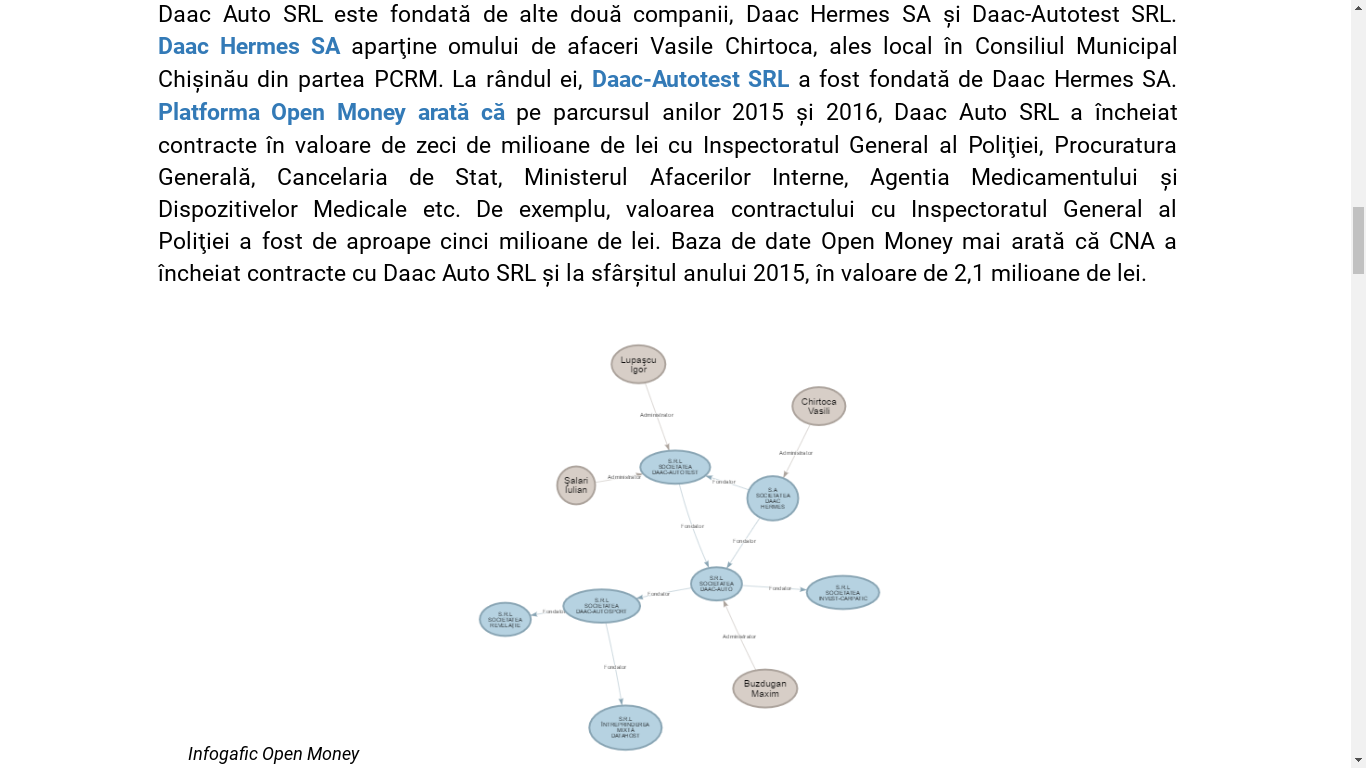
\includegraphics[width=17cm]{ac1.png} 
	\caption{ Part of \underline{anticoruptie.md}'s article - "Achiziţiile CNA // Şase maşini Skoda Rapid, cumpărate cu 1,5 milioane de lei" }\label{fig4} 
	\end{figure}
	
\item "Proprietarii site-urilor de ştiri şi interesele pe care le promovează".

In this article platform is used to show real founders of a website of news "Noi.md". This website was founded by the "MLD Media SRL" company, but the company is founded directly by some persons and companies. In this case platform is used to identify indirect founders that stay from behind of direct founding companies, using foundation hierarchy of company feature in Figure 5.2 is very simple to find them all. One of these persons is "Vasile Chirtoca" - politician from PCRM. In result was found a indirect relation between a politician and website of news.\\
	\begin{figure}[!ht] 
	\renewcommand\thefigure{5.2} % Make this Figure I.3 
	\centering 
	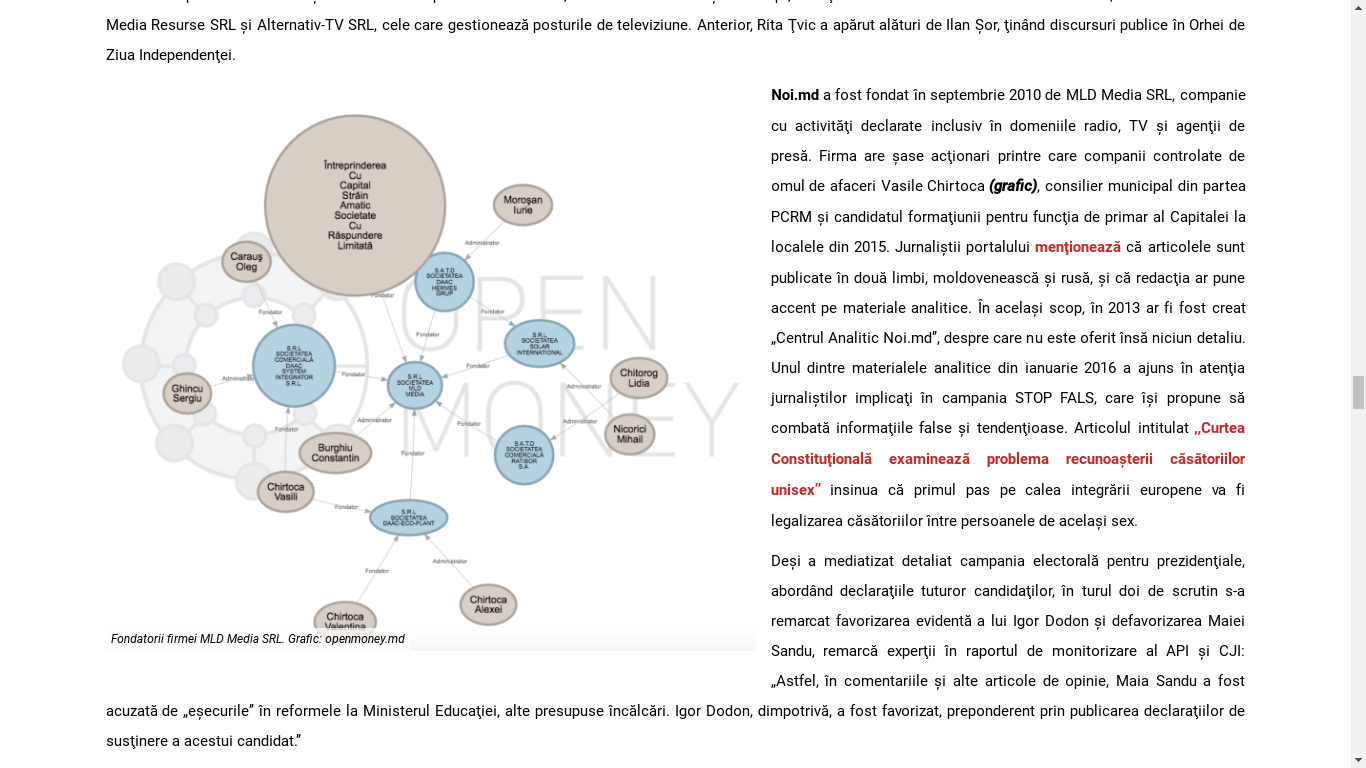
\includegraphics[width=17cm]{ac2.png} 
	\caption{ Part of \underline{anticoruptie.md}'s article - "Proprietarii site-urilor de ştiri şi interesele pe care le promovează" }\label{fig4} 
	\end{figure}
	
\item "Moratoriu de ochii lumii. Cine construiește benzinării în Capitală"

In this investigation of gas stations in Chisinau platform is used to show hierarchy of ownership/founding of a gas station company - "Luconex SRL", check Figure 5.3.

\begin{figure}[!ht] 
	\renewcommand\thefigure{5.3} % Make this Figure I.3 
	\centering 
	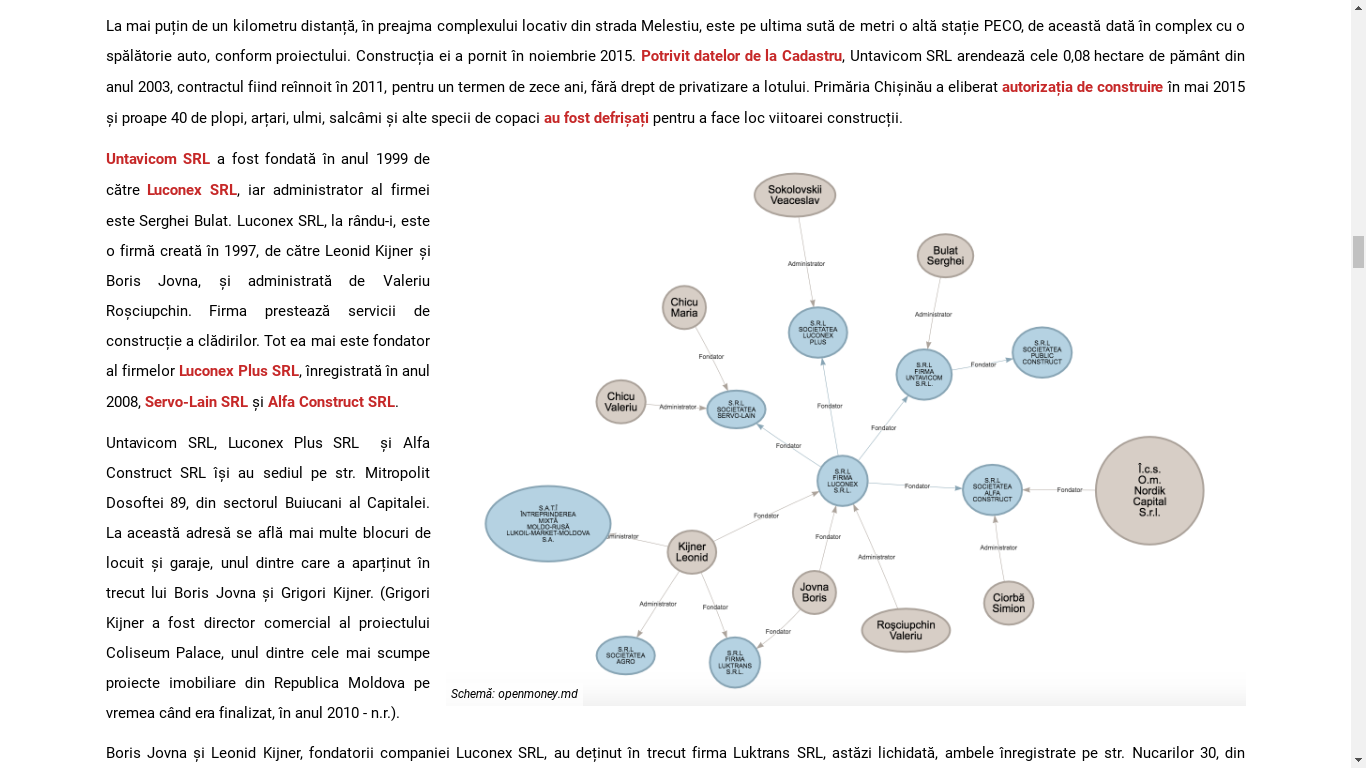
\includegraphics[width=17cm]{ac3.png} 
	\caption{ Part of \underline{anticoruptie.md}'s article - "Moratoriu de ochii lumii. Cine construiește benzinării în Capitală" }\label{fig4} 
	\end{figure}

\end{itemize}


 

\newpage
\phantomsection
\addcontentsline{toc}{section}{Conclusions}
\section*{Conclusions}

	After release of project platform was already used by some news websites like anticoruptie.md, agora.md and others in about 5-10 investigation articles mentioned in section ahead.
	
	 Main problem in implementing of project was quality of data exposed by government website, every type of data has lack of ID, so linking between entities occured by name, there comes another problem, the names from different XLS files may differ, for example in one file "Universitatea tehnica din Moldova" but in another "Universitatea tehnica a Moldovei", so was applied some additional techniques for similarity matching like "levenshtein distance" and others. Also another problem in those data is unstable schema, older and new data differ by structure in more versions that creates.

Next major feature in application is to add versioning of graph states in time, for that moment is only the state for last quarter data.
	 
	
	From technological point of view in this project were many challenges. First problem was decision of general architecture for system. This platform is form-intensive, so it is ideally suited for being built as single page web application. The main idea compared to other more traditional server-side architectures is to build the server as a stateless reusable REST service. In such a way project take advantage of decoupling client part from server, which means a separation between development teams for each part and a faster implementation because of focusing on separate things with intersection just in synchronization of interface of communication (REST API). For client part we had to choose between two frameworks: AngularJS and Aurelia, both are top used frameworks, but client is part with low priority attention, so decision was based on the fact that AngularJS is more generalist with overhead of configuration stuff, but with Aurelia development occured much faster. Part with a higher priority was server. From this part decision was first of all around which database management system to use for project's purposes. As earlier was discussed that the key point of the project is representation of all entities(persons, companies institutions) and relations(administration, founding, acquisitions between company and institution) in form of graph model, so i decided to choose a NoSQL DBMS of graph type that supports that graph model in persistent context. Such a technology has well defined things like storage management, performance, specific algorithms in its own engine for graph model, so it make much easier to implement business logic for features related to data processing in graph context. Decision was between two implementations of such DBMS type: OrientDB and Neo4j. In result the obvious winner for my purposes was OrientDB for next reasons:
\begin{itemize}
\item OrientDB supports Multi-Model concept (graph, documents, objects, key-values), Neo4j supports only graph model
\item Performance - According to an independent benchmark by Tokyo Institute of Technology* and IBM Research*, OrientDB is 10X faster than Neo4j* on Graph operations among all the workloads
\item Available features in Community Edition are more limited in Neo4j
\item Declarative way of interaction in OrientDB is SQL like with graph related extension, which is more familiar than Neo4j's "Cypher" query language which is totally a new kind of language for me, so need more time to learn it.
\end{itemize}	 
As server-side application language does not matter so much, for much of them exists driver from OrientDB vendor. As i am familiar wih Java i have choosen it. From frameworks i have choosen ones from most popular ecosystem for enterprise solutions - "Spring" stack, Spring Core as dependency injection library and Spring MVC as web layer for request intercepting. Reason of course is large community support.

\cleardoublepage

\newpage
\phantomsection
\addcontentsline{toc}{section}{References}
\begin{thebibliography}{99999}

\bibitem{Spring in Action} Craig Walls, \textit{Spring in action}, \url{https://www.manning.com/books/spring-in-action-fourth-edition}, (April 4 2017)
\bibitem{Do-factory-design-patterns} Data \& Object Factory, LLC., \textit{.NET Design patterns}, \url{http://www.dofactory.com/net/design-patterns}, (April 6 2017)
\bibitem{Java-DIF-options} Shannon Griswold, \textit{Dependency Injection Options for Java}, \url{https://keyholesoftware.com/2014/02/17/dependency-injection-options-for-java/}, (April 6 2017)
\bibitem{Java-setter-vs-constructor} Alef Arendsen, \textit{Setter injection versus constructor injection and the use of @Required}, \url{https://spring.io/blog/2007/07/11/setter-injection-versus-constructor-injection-and-the-use-of-required/}, (April 8 2017)
\bibitem{oodesign-factory} oodesign.com, \textit{Factory Pattern}, \url{http://www.oodesign.com/factory-pattern.html}, (April 10 2017)
\bibitem{gof} Erich Gamma, Richard Helm, Ralph Johnson, John Vlissides, \textit{Design Patterns: Elements of Reusable Object-Oriented Software}, USA, Addison-Wesley, 1994, chapters 6, pages 416
\bibitem{tutorialspoint-prototype} tutorialspoint.com, \textit{Design Patterns - Prototype Pattern}, \url{https://www.tutorialspoint.com/design_pattern/prototype_pattern.htm}, (April 11 2017)
\bibitem{spring-scopes} Pivotal Software, \textit{Request, session, global session, application, and WebSocket scopes}, \url{https://docs.spring.io/spring/docs/current/spring-framework-reference/htmlsingle/#beans-factory-scopes-other}, (April 20 2017)
\bibitem{spring-framework} Pivotal Software, \textit{Spring framework}, \url{https://projects.spring.io/spring-framework/}, (April 22 2017)


\end{thebibliography}
\cleardoublepage
    
    
\end{document}
